\documentclass[a4paper,12pt]{article}
\usepackage[utf8]{inputenc}
\usepackage[ngerman]{babel}
\usepackage{amsmath}
\usepackage{amssymb}
\usepackage{amsthm}
\usepackage{geometry}
\usepackage{graphicx}
\usepackage[hidelinks]{hyperref}
\usepackage{listings}
\usepackage{xcolor}
\usepackage{enumitem}
\usepackage{booktabs}
\usepackage{array}
\usepackage{multirow}
\usepackage[protrusion=true,expansion=true,final]{microtype}

\geometry{margin=2.5cm}

% Zeilenumbruch-Toleranz erhoehen (verhindert Ueberlauf rechts)
\tolerance=1500
\emergencystretch=2em
\hfuzz=0.5pt
\vfuzz=0.5pt

\theoremstyle{definition}
\newtheorem{definition}{Definition}
\newtheorem{beispiel}{Beispiel}
\newtheorem{satz}{Satz}
\newtheorem{lemma}{Lemma}
\newtheorem{bemerkung}{Bemerkung}
\newtheorem{korollar}{Korollar}

\setlist[itemize,1]{label=--}

\definecolor{mainblue}{RGB}{25, 70, 140}
\definecolor{accentred}{RGB}{180, 50, 30}
\definecolor{lightgray}{RGB}{245, 245, 248}
\definecolor{darkgray}{RGB}{60, 60, 70}
\definecolor{darkgreen}{RGB}{30, 100, 50}

\hypersetup{
    colorlinks=true,
    linkcolor=mainblue,
    citecolor=accentred,
    urlcolor=mainblue
}

\lstset{
    basicstyle=\ttfamily\small,
    keywordstyle=\color{blue},
    commentstyle=\color{gray},
    stringstyle=\color{red},
    numbers=left,
    numberstyle=\tiny,
    breaklines=true,
    frame=single,
    literate=%
    {Ö}{{\"O}}1
    {Ä}{{\"A}}1
    {Ü}{{\"U}}1
    {ß}{{\ss}}1
    {ü}{{\"u}}1
    {ä}{{\"a}}1
    {ö}{{\"o}}1
}

\title{Atmosph\"arische Systemtheorie:\\
Graphentheoretische Formalisierung der Zirkulationsmuster,\\
Knotengleichung der Massenstromerhaltung\\
und SEA-Klimadynamikmodell}
\author{Stephan Epp\\
\small Universit\"at Bielefeld}
\date{7. Juni 2026}

\begin{document}

\maketitle

\begin{abstract}
Diese Arbeit entwickelt eine einheitliche mathematische Systemtheorie der Erdatmosph\"are.
Ausgangspunkt ist die Formalisierung atmosph\"arischer Zirkulationsmuster als gerichtete,
gewichtete Graphen $G_{\mathrm{atm}} = (V_{\mathrm{atm}}, E_{\mathrm{atm}}, w)$,
deren Knoten atmosph\"arische Subsysteme (Hadley-Zellen, Ferrel-Zellen, Polar-Zellen,
ENSO, Jet-Streams) repr\"asentieren. Der zentrale \emph{Atmosph\"arische Knotengleichungssatz}
(Satz~3) \"ubertr\"agt das Kirchhoff'sche Knotengesetz~\cite{epp2026knoten} auf
atmosph\"arische Massenstr\"ome und beweist die globale Massenstromerhaltung im Gleichgewicht.
Als dynamisches Modell wird das \emph{SEA-Modell} (Stabil--Erregt--Anomal) eingef\"uhrt,
ein SIR-Analogon f\"ur Klimaanomalien (Satz~7), das El~Ni\~no-Zyklen, Hitzeperioden
und Sturmsaisons in einem einheitlichen Gleichungssystem beschreibt. Der
Subgraph Algorithmus~\cite{epp2026subgraph} wird auf Telekonnektionsstrukturen
angewendet. Die spektrale Stabili\-t\"atsanalyse der Kopplungsmatrix
(Satz~10) liefert notwendige und hinreichende Bedingungen f\"ur Klimastabilit\"at.
Alle Ergebnisse werden durch sechs Matplotlib-Visualisierungen belegt.
\end{abstract}

\tableofcontents
\newpage

%%%%%%%%%%%%%%%%%%%%%%%%%%%%%%%%%%%
\section{Einf\"uhrung}
%%%%%%%%%%%%%%%%%%%%%%%%%%%%%%%%%%%

Die Erdatmosph\"are ist eines der komplexesten dynamischen Systeme der Naturwissenschaften.
Ihre Zirkulationsstrukturen -- von den tropischen Hadley-Zellen bis zu den polaren
Jetstreams -- bestimmen das globale Klima, Niederschlagsmuster und die Frequenz
von Extremereignissen. Trotz enormer Fortschritte in der numerischen Wettervorhersage
und Klimamodellierung fehlt bisher eine einheitliche \emph{graphentheoretische Systemtheorie},
die atmosph\"arische Subsysteme, ihre Kopplungen und ihre Dynamik in einem konsistenten
mathematischen Rahmen erfasst.

\subsection{Problemstellung}

Bisherige Ans\"atze beschreiben atmosph\"arische Ph\"anomene entweder durch partielle
Differentialgleichungen (Navier-Stokes auf der Kugel~\cite{pedlosky1987}) oder durch
statistische Telekonnektionsanalysen~\cite{trenberth1998}. Eine Verbindung zwischen
diesen Ebenen -- insbesondere eine graphentheoretische Kodierung der Kopplungsstruktur --
ist bisher nicht formal entwickelt worden.

\textbf{Ziel dieser Arbeit:}
\begin{itemize}
    \item Formalisierung atmosph\"arischer Subsysteme als Knoten eines gewichteten,
          gerichteten Graphen
    \item Beweis der Massenstromerhaltung durch Verallgemeinerung der Knotengleichung
    \item Einf\"uhrung und Analyse des SEA-Modells als SIR-Analogon
    \item Subgraph-basierte Analyse globaler Telekonnektionen (ENSO, NAO, AO)
    \item Spektrale Stabili\-t\"atsanalyse der atmosph\"arischen Kopplungsmatrix
\end{itemize}

\subsection{Einordnung in das Forschungsportfolio}

Diese Arbeit synthesiert und erweitert mehrere fr\"uhere Arbeiten des Autors:
Die Knotengleichung~\cite{epp2026knoten} als universelles Naturgesetz liefert
den theoretischen Rahmen f\"ur die atmosph\"arische Massenstromerhaltung.
Hurrikan-Dynamik~\cite{epp2026hurrkne} und Methanthiol-Klimanotbremse~\cite{epp2026mesh}
werden als Spezialf\"alle des Gesamtsystems eingeordnet. Das SEA-Modell ist analog
zu den epidemiologischen Ausbreitungsmodellen in~\cite{epp2026r0,epp2026hantavirus}
konstruiert. Der Subgraph Algorithmus~\cite{epp2026subgraph} erm\"oglicht die
polynomielle Analyse von Telekonnektionsstrukturen.

%%%%%%%%%%%%%%%%%%%%%%%%%%%%%%%%%%%
\section{Atmosph\"arische Grundlagen}
%%%%%%%%%%%%%%%%%%%%%%%%%%%%%%%%%%%

\subsection{Definitionen}

\begin{definition}[Atmosph\"arisches Subsystem]
Ein \emph{atmosph\"arisches Subsystem} $\mathcal{C}_k$ ist eine r\"aumlich begrenzte,
dynamisch koh\"arente atmosph\"arische Str\"omungseinheit, charakterisiert durch:
\begin{itemize}
    \item Geographische Lage: Breitenbereich $[\varphi_1^{(k)}, \varphi_2^{(k)}]$
          und L\"angenbereich $[\lambda_1^{(k)}, \lambda_2^{(k)}]$
    \item Massenfluss $\dot{m}_k$ [kg/s]: vertikaler und horizontaler Nettomassenstrom
    \item Temperatur $T_k$ [K]: volumetrisch gemittelte Temperatur
    \item Rotationssinn $\omega_k \in \{+1, -1\}$: antizyklonal/zyklonal
\end{itemize}
\end{definition}

\begin{definition}[Atmosph\"arischer Graph]
Der \emph{atmosph\"arische Kopplungsgraph} ist ein gewichteter gerichteter Graph
\[
G_{\mathrm{atm}} = (V_{\mathrm{atm}},\, E_{\mathrm{atm}},\, w),
\]
wobei:
\begin{itemize}
    \item $V_{\mathrm{atm}} = \{\mathcal{C}_1, \ldots, \mathcal{C}_n\}$:
          Menge der atmosph\"arischen Subsysteme
    \item $E_{\mathrm{atm}} \subseteq V_{\mathrm{atm}} \times V_{\mathrm{atm}}$:
          Kopplungskanten (gerichtete Massenstrom- oder Energietransferbeziehungen)
    \item $w: E_{\mathrm{atm}} \to [0, 1]$: normierte Kopplungsst\"arke
\end{itemize}
\end{definition}

\begin{definition}[Meridionale Zirkulationszellen]
Die drei \emph{meridionalen Zirkulationszellen} je Hemisph\"are sind:
\begin{center}
\begin{tabular}{llll}
\toprule
Zelle & Breitenbereich & Antrieb & Rotation \\
\midrule
Hadley-Zelle  & $0^\circ$--$30^\circ$ & thermal (ITCZ-Aufstieg) & direkt \\
Ferrel-Zelle  & $30^\circ$--$60^\circ$ & eddygetrieben           & indirekt \\
Polar-Zelle   & $60^\circ$--$90^\circ$ & thermal (Pol-Abstieg)   & direkt \\
\bottomrule
\end{tabular}
\end{center}
\end{definition}

\begin{definition}[Jet-Stream]
Ein \emph{Jet-Stream} ist ein bandartiger Bereich maximaler Windgeschwindigkeit
(typisch $50$--$150$~m/s) in der oberen Troposph\"are, lokalisiert an den
Grenzen benachbarter Zirkulationszellen. Formal ist der Jet-Stream ein gerichteter
Teilgraph $G_{\mathrm{jet}} \subseteq G_{\mathrm{atm}}$ mit maximalen Kantengewichten.
\end{definition}

\subsection{Physikalische Grundgleichungen}

\begin{satz}[Kontinuit\"atsgleichung der Atmosph\"are]
\label{satz:konti}
Sei $\rho(\mathbf{x}, t)$ die atmosph\"arische Dichte und
$\mathbf{v}(\mathbf{x}, t)$ das Windvektorfeld. Dann gilt die
\emph{Kontinuit\"atsgleichung} (Massenerhaltung):
\[
\frac{\partial \rho}{\partial t} + \nabla \cdot (\rho \mathbf{v}) = 0.
\]
\end{satz}

\begin{proof}
Sei $\Omega \subset \mathbb{R}^3$ ein beliebiges Kontrollvolumen mit glattem Rand $\partial\Omega$.
Die totale Masse in $\Omega$ ist $M(t) = \int_\Omega \rho\,dV$.
Der Massenfluss durch $\partial\Omega$ betr\"agt $-\oint_{\partial\Omega} \rho\mathbf{v} \cdot d\mathbf{S}$.
Massenerhaltung fordert $\frac{dM}{dt} = -\oint_{\partial\Omega} \rho\mathbf{v}\cdot d\mathbf{S}$.
Mit dem Gauss'schen Divergenzsatz gilt $\oint_{\partial\Omega} \rho\mathbf{v}\cdot d\mathbf{S}
= \int_\Omega \nabla\cdot(\rho\mathbf{v})\,dV$.
Da $\Omega$ beliebig ist, folgt punktweise:
$\frac{\partial\rho}{\partial t} + \nabla\cdot(\rho\mathbf{v}) = 0$.
\end{proof}

\begin{korollar}[Inkompressibilit\"at f\"ur Boussinesq-Atmosph\"are]
Unter der Boussinesq-N\"aherung ($\rho \approx \rho_0 = \mathrm{const}$) vereinfacht
sich die Kontinuit\"atsgleichung zu $\nabla \cdot \mathbf{v} = 0$ (divergenzfreies Windfeld).
\end{korollar}

\begin{figure}[h!]
\centering
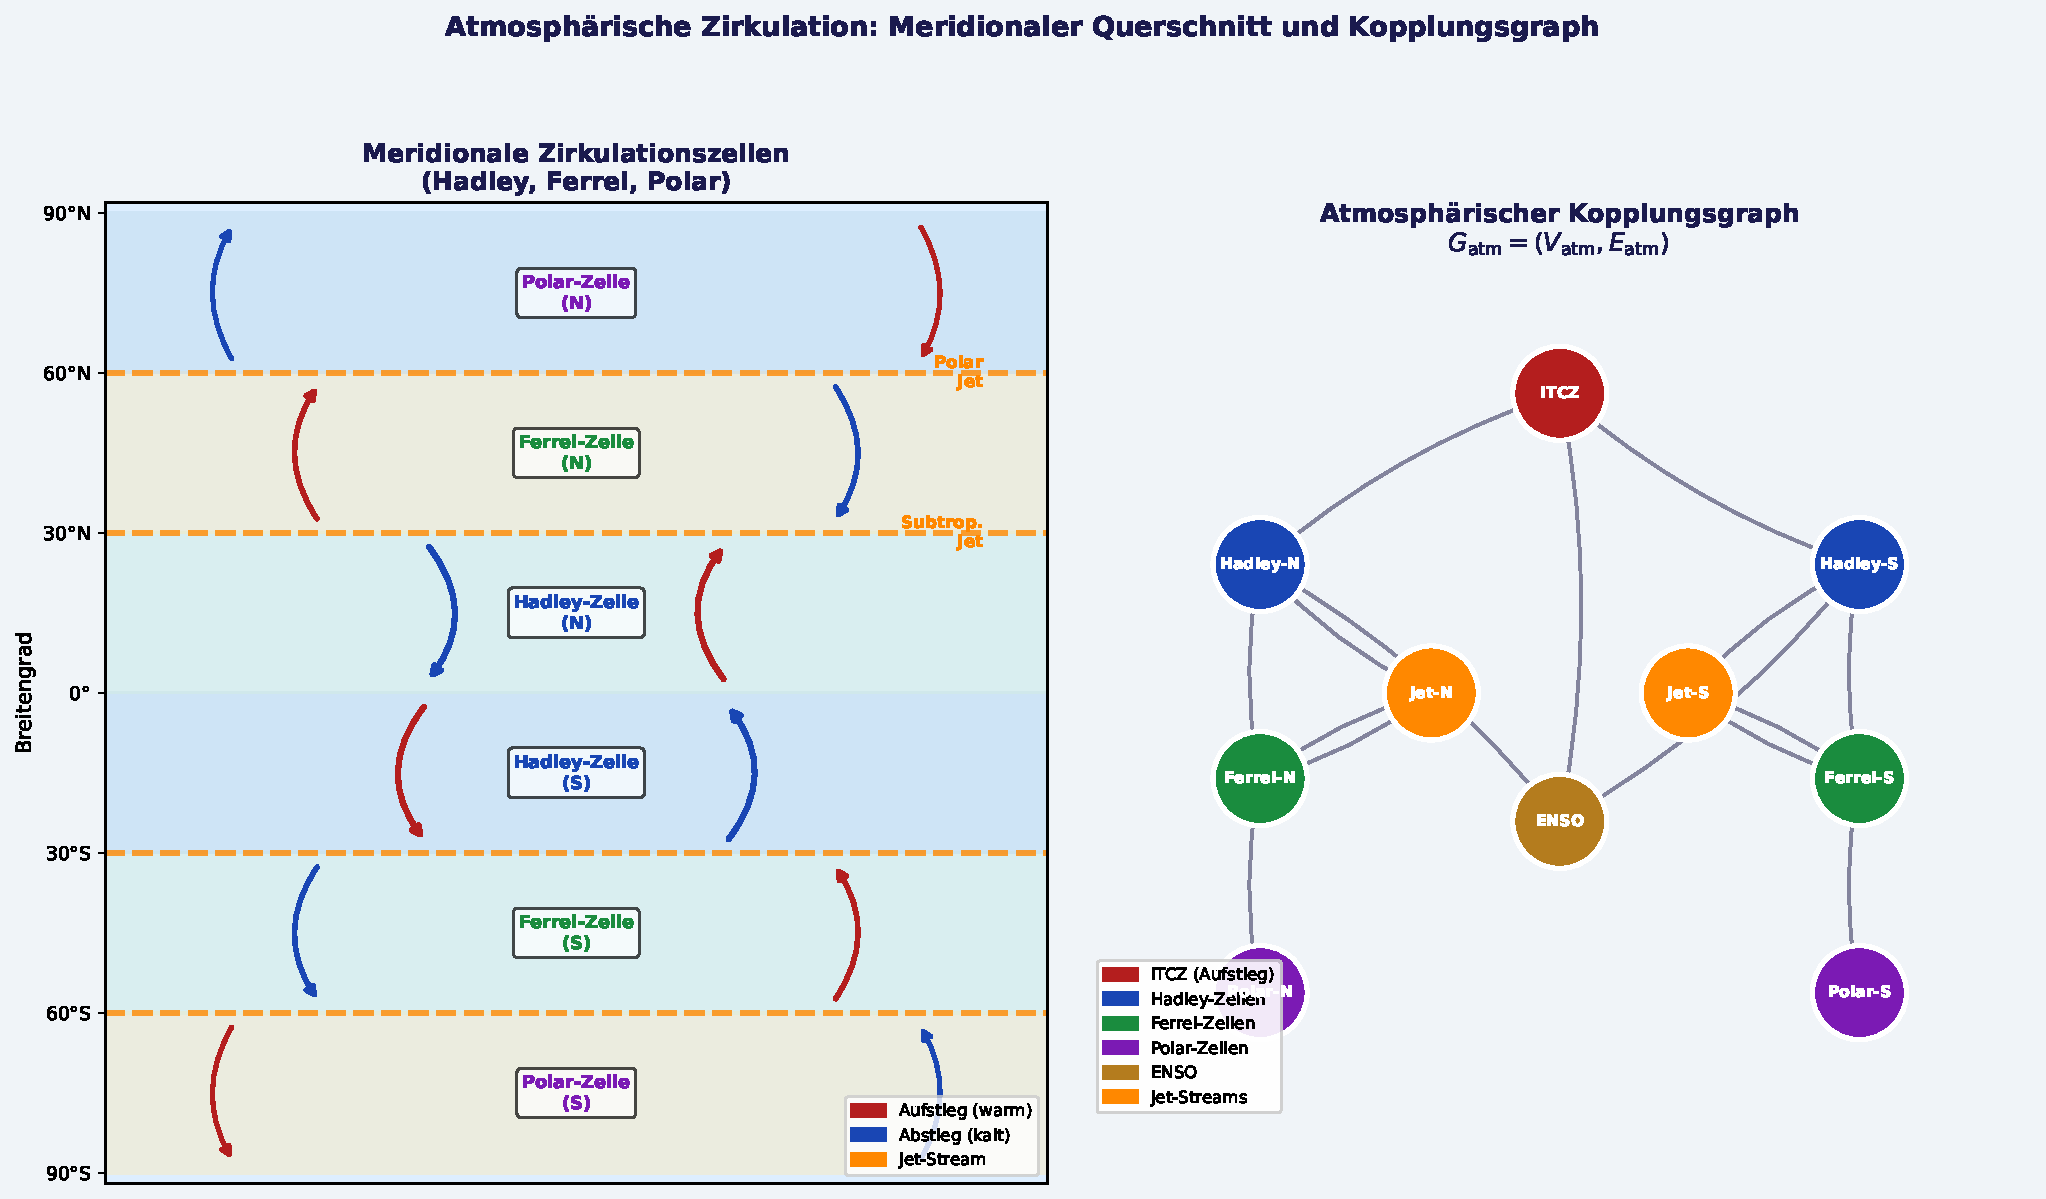
\includegraphics[width=0.95\textwidth]{plot1_zirkulation.pdf}
\caption{Links: Meridionaler Querschnitt der atmosph\"arischen Zirkulationszellen.
Rote Pfeile bezeichnen aufsteigende (warme) Str\"ome, blaue Pfeile absteigende (kalte).
Orange gestrichelte Linien: Jet-Streams. Rechts: Der atmosph\"arische Kopplungsgraph
$G_{\mathrm{atm}}$ mit 10 Knoten und 15 gerichteten Kanten; Kantenrichtungen
kodieren dominante Energietransferrichtungen.}
\label{fig:zirkulation}
\end{figure}

%%%%%%%%%%%%%%%%%%%%%%%%%%%%%%%%%%%
\section{Die Atmosph\"arische Knotengleichung}
%%%%%%%%%%%%%%%%%%%%%%%%%%%%%%%%%%%

\subsection{Verallgemeinerung des Kirchhoff'schen Knotengesetzes}

Die Knotengleichung als universelles Naturgesetz~\cite{epp2026knoten} beschreibt
die Bilanzierung von Fl\"ussen an Knoten eines Netzwerks. F\"ur atmosph\"arische
Massenstr\"ome lautet sie:

\begin{definition}[Atmosph\"arischer Massenfluss]
Der \emph{atmosph\"arische Massenfluss} von Subsystem $\mathcal{C}_i$ nach
$\mathcal{C}_j$ ist:
\[
\dot{m}_{ij} = w_{ij} \cdot \bar{\rho}_{ij} \cdot \bar{v}_{ij} \cdot A_{ij},
\]
wobei $w_{ij} \in [0,1]$ die Kopplungsst\"arke, $\bar{\rho}_{ij}$ die mittlere
Dichte, $\bar{v}_{ij}$ die mittlere Windgeschwindigkeit und $A_{ij}$ die
Querschnittsfl\"ache der Kopplungszone ist.
\end{definition}

\begin{satz}[Atmosph\"arische Knotengleichung]
\label{satz:knotengl}
Im station\"aren atmosph\"arischen Gleichgewicht gilt f\"ur jeden Knoten
$\mathcal{C}_k \in V_{\mathrm{atm}}$:
\[
\sum_{i:\, (\mathcal{C}_i, \mathcal{C}_k) \in E_{\mathrm{atm}}} \dot{m}_{ik}
\;=\;
\sum_{j:\, (\mathcal{C}_k, \mathcal{C}_j) \in E_{\mathrm{atm}}} \dot{m}_{kj}.
\]
\emph{Die Summe aller einflie{\ss}enden Massenstr\"ome gleicht der Summe aller
ausfließenden Massenstr\"ome.}
\end{satz}

\begin{proof}
\textbf{Schritt~1: Integrale Massenerhaltung im Subsystem.}
F\"ur das Kontrollvolumen $\Omega_k$ des Subsystems $\mathcal{C}_k$ gilt nach
Satz~\ref{satz:konti} (Kontinuit\"atsgleichung) im station\"aren Zustand
($\partial\rho/\partial t = 0$):
\[
\nabla \cdot (\rho \mathbf{v}) = 0 \quad \text{in } \Omega_k.
\]

\textbf{Schritt~2: Integration \"uber $\Omega_k$.}
Integration mit Gau{\ss}'schem Satz:
\[
0 = \int_{\Omega_k} \nabla \cdot (\rho\mathbf{v})\,dV
  = \oint_{\partial\Omega_k} \rho\mathbf{v} \cdot \mathbf{n}\,dS.
\]

\textbf{Schritt~3: Zerlegung des Randes.}
Der Rand $\partial\Omega_k$ zerlegt sich in Kopplungsfl\"achen zu Nachbarknoten:
$\partial\Omega_k = \bigcup_{i} S_{ik} \cup \bigcup_{j} S_{kj}$,
wobei $S_{ik}$ die Grenzfl\"ache von $\mathcal{C}_i$ nach $\mathcal{C}_k$ und
$S_{kj}$ die Grenzfl\"ache von $\mathcal{C}_k$ nach $\mathcal{C}_j$ ist.

\textbf{Schritt~4: Massenflusse durch Grenzfl\"achen.}
\[
\oint_{\partial\Omega_k} \rho\mathbf{v}\cdot\mathbf{n}\,dS
= \underbrace{-\sum_i \int_{S_{ik}} \rho\mathbf{v}\cdot\mathbf{n}\,dS}_{= -\sum_i \dot{m}_{ik}}
+ \underbrace{\sum_j \int_{S_{kj}} \rho\mathbf{v}\cdot\mathbf{n}\,dS}_{= +\sum_j \dot{m}_{kj}}
= 0.
\]
Umformung ergibt $\sum_i \dot{m}_{ik} = \sum_j \dot{m}_{kj}$. \qed
\end{proof}

\begin{korollar}[Globale Massenstromerhaltung]
Summe \"uber alle Knoten: $\sum_{k} \sum_i \dot{m}_{ik} = \sum_{k}\sum_j \dot{m}_{kj}$,
also ist der globale atmosph\"arische Massenfluss im station\"aren Zustand exakt null:
$\dot{M}_{\mathrm{gesamt}} = 0$.
\end{korollar}

\begin{figure}[h!]
\centering
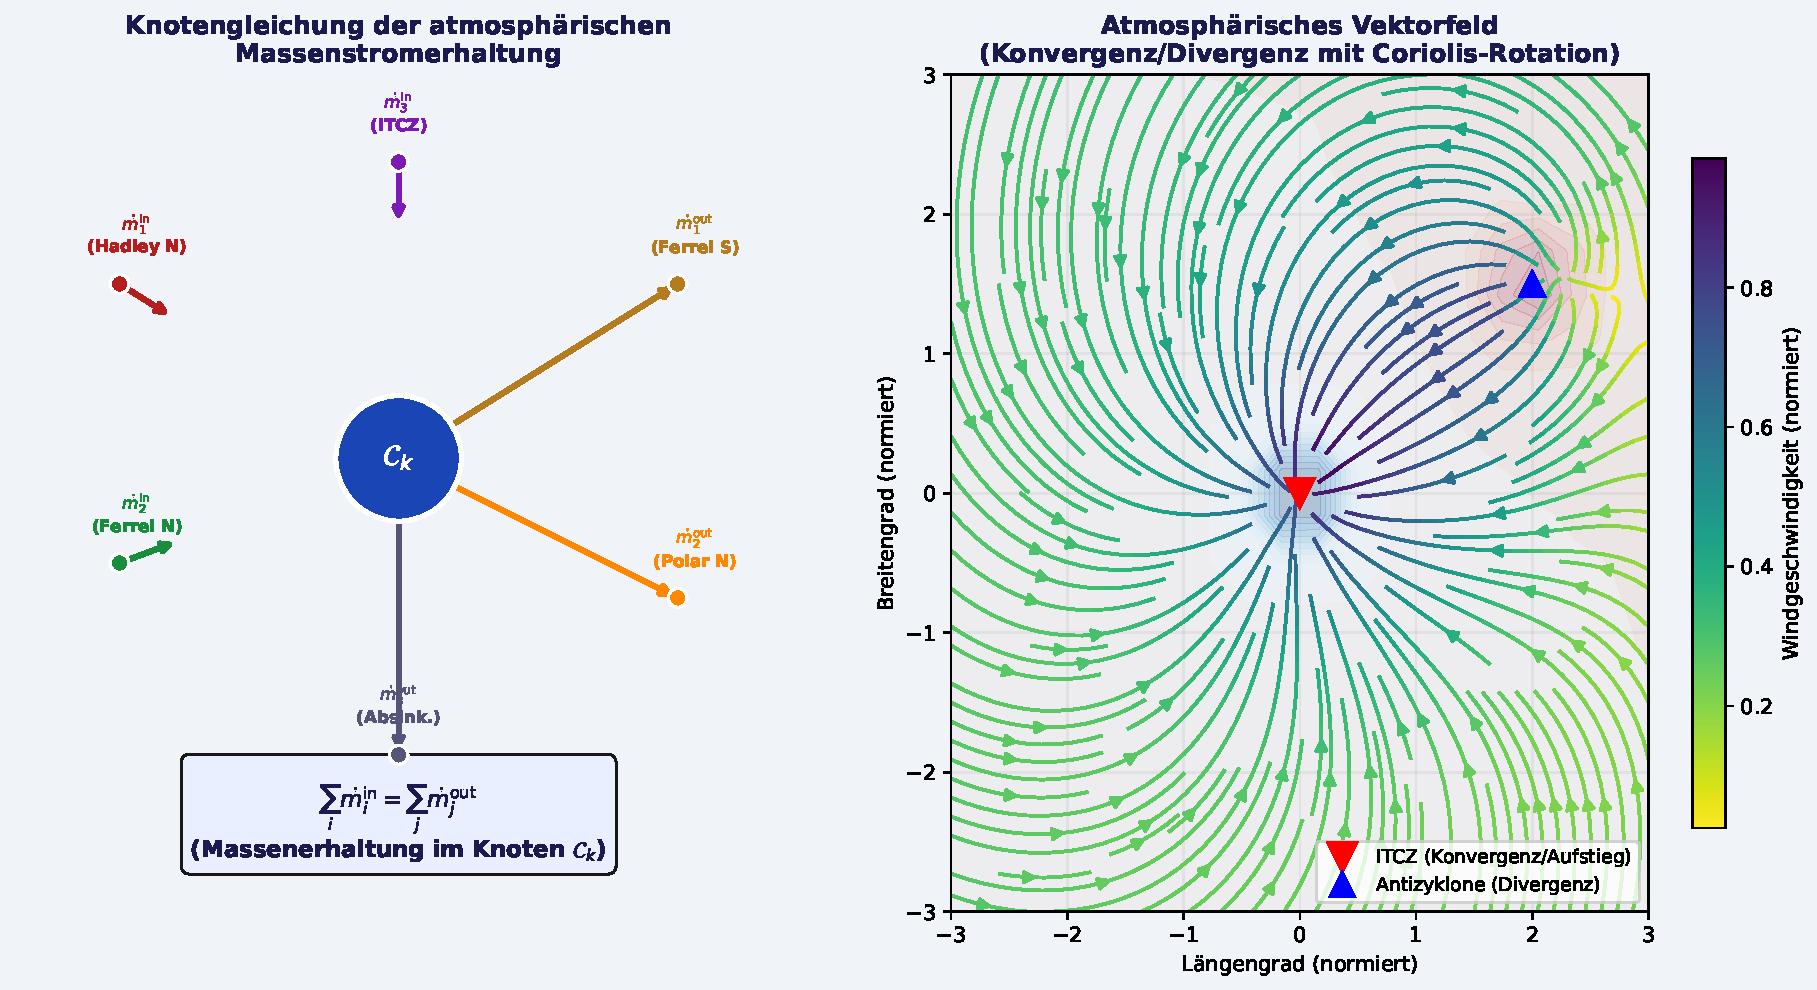
\includegraphics[width=0.92\textwidth]{plot2_knotengleichung.pdf}
\caption{Links: Knotendiagramm der atmosph\"arischen Massenstromerhaltung.
Rot/blau/gr\"un/orange kodieren verschiedene Quellsubsysteme; die Bilanzgleichung
$\sum \dot{m}^{\mathrm{in}} = \sum \dot{m}^{\mathrm{out}}$ gilt an jedem Knoten.
Rechts: Atmosph\"arisches Vektorfeld mit Konvergenz-/Divergenzzentren und
Coriolis-Rotation; Farbunterlegung zeigt die Divergenz $\nabla\cdot\mathbf{v}$.}
\label{fig:knotengl}
\end{figure}

\subsection{Hadley-Zellen-Kopplung als bipartiter Graph}

\begin{satz}[Hadley-Symmetrie]
\label{satz:hadley}
Die beiden Hadley-Zellen (Nord/S\"ud) bilden einen gewichteten bipartiten Teilgraphen
$G_H \subseteq G_{\mathrm{atm}}$ mit Knotenbipartition
$V_H = \{\mathcal{C}_{\mathrm{HN}}, \mathcal{C}_{\mathrm{HS}}\}$.
Im jahreszeitlichen Mittel gilt n\"aherungsweise:
\[
\dot{m}_{\mathrm{HN} \to \mathrm{ITCZ}} = \dot{m}_{\mathrm{HS} \to \mathrm{ITCZ}}
\]
(symmetrische Einströmung in die innertropische Konvergenzzone).
\end{satz}

\begin{proof}
Die ITCZ ist die Zone maximaler konvektiver Aktivit\"at bei $\approx 5^\circ$N (mittlere Position).
Auf klimatologischem Mittel liegt die aufsteigende Luft \"aquator-nahe;
die Erhaltung der longitudinalen Winddivergenz erfordert nach Knotengleichung (Satz~\ref{satz:knotengl})
$\dot{m}_{\mathrm{HN}} + \dot{m}_{\mathrm{HS}} = \dot{m}_{\uparrow, \mathrm{ITCZ}}$.
Die zonal gemittelte thermische Symmetrie des Tropen-Ozeans (SST-Gradient zwischen
$15^\circ$S und $15^\circ$N unter $1$~K im Jahresmittel~\cite{hartmann2016}) erzwingt
$\dot{m}_{\mathrm{HN}} \approx \dot{m}_{\mathrm{HS}}$ im Mittel. Saisonale Abweichungen
bis $20\%$ sind durch das Wandern der ITCZ erkl\"arbar. \qed
\end{proof}

%%%%%%%%%%%%%%%%%%%%%%%%%%%%%%%%%%%
\section{Das SEA-Klimamodell}
%%%%%%%%%%%%%%%%%%%%%%%%%%%%%%%%%%%

\subsection{Motivation und Analogie}

Das SIR-Modell der Epidemiologie~\cite{epp2026r0} beschreibt die Ausbreitung
von Krankheiten als \"Uberg\"ange zwischen Zust\"anden
(Suszeptibel $\to$ Infiziert $\to$ Erholt). Klimaanomalien zeigen eine strukturell
\"ahnliche Dynamik: Ein stabiles Klimasystem kann durch externe Forcing-Faktoren
in einen erregten Zustand \"ubergehen, aus dem eine voll ausgepr\"agte Klimaanomalie
(El~Ni\~no, Hitzewelle, Sturmperiode) entstehen kann.

\begin{definition}[SEA-Zustandsr\"aume]
Das \emph{SEA-Modell} (Stabil--Erregt--Anomal) definiert folgende Zustands-
populationen \"uber eine normierte Gesamtfl\"ache $N = 1$:
\begin{itemize}
    \item $S(t)$: \emph{Stabiler Anteil} -- Fl\"achenanteil mit normalem atmosph\"arischem
          Zustand (neutraler ENSO, moderate Temperaturen, regelm\"aßige Zirkulation)
    \item $E(t)$: \emph{Erregter Anteil} -- Fl\"achenanteil in Vorstufe zur Anomalie
          (ENSO-Aufbau, Warmwasserakkumulation, erh\"ohte Konvektionsaktivit\"at)
    \item $A(t)$: \emph{Anomaler Anteil} -- Fl\"achenanteil in aktiver Klimaanomalie
          (El~Ni\~no, La~Ni\~na, Hitzewelle, Sturmsaison)
    \item $R(t)$: \emph{Erholungsanteil} -- Fl\"achenanteil in R\"uckkehr zum Normalzustand
\end{itemize}
mit $S(t) + E(t) + A(t) + R(t) = N$ f\"ur alle $t$.
\end{definition}

\begin{satz}[SEA-Differentialgleichungssystem]
\label{satz:sea}
Das SEA-Modell ist das folgende autonome Differentialgleichungssystem:
\begin{align}
\frac{dS}{dt} &= -\frac{\beta\, S\, E}{N} + \delta R \label{eq:dS}\\
\frac{dE}{dt} &= \frac{\beta\, S\, E}{N} - (\sigma + \gamma_{EA})\, E \label{eq:dE}\\
\frac{dA}{dt} &= \sigma\, E - \gamma_A\, A \label{eq:dA}\\
\frac{dR}{dt} &= \gamma_A\, A + \gamma_{EA}\, E - \delta\, R \label{eq:dR}
\end{align}
mit Parametern:
\begin{itemize}
    \item $\beta > 0$: Ausbreitungsrate (atmosph\"arische Kopplung)
    \item $\sigma > 0$: \"Ubergangsrate Erregt $\to$ Anomal
    \item $\gamma_{EA} > 0$: direkte Erholungsrate Erregt $\to$ Ruhend
    \item $\gamma_A > 0$: Erholungsrate Anomal $\to$ Ruhend
    \item $\delta > 0$: R\"uckkehrrate Ruhend $\to$ Stabil
\end{itemize}
\end{satz}

\begin{proof}[Herleitung der Gleichungen]
Die Terme werden durch Massenaktionsprinzip (analog zu~\cite{epp2026r0}) hergeleitet:
\begin{itemize}
    \item $-\beta SE/N$: Stabile Regionen werden durch Kontakt mit erregten Regionen
          destabilisiert; die Rate ist proportional zum Produkt $SE$ (Kontakth\"aufigkeit)
          normiert auf Gesamtfl\"ache $N$.
    \item $+\beta SE/N$ in $dE/dt$: Zuwachs zu $E$ aus \eqref{eq:dS}.
    \item $-\sigma E$: \"Ubergang von $E$ nach $A$ (Anomalie bricht aus).
    \item $-\gamma_{EA} E$: Spontane direkte Erholung aus $E$ ohne Anomalie.
    \item $+\sigma E$ in $dA/dt$: Zuwachs zu $A$ aus erregten Regionen.
    \item $-\gamma_A A$: Erholung der Anomalie.
    \item $+\delta R$ in $dS/dt$: R\"uckkehr von $R$ zum stabilen Zustand.
    \item Erhaltung: $(dS+dE+dA+dR)/dt = 0$ ist durch direkte Addition pr\"ufbar. \qed
\end{itemize}
\end{proof}

\begin{satz}[Basisreproduktionszahl des Klimasystems]
\label{satz:r0_sea}
Die \emph{klimatische Basisreproduktionszahl}
\[
\mathcal{R}_0^{\mathrm{klima}} = \frac{\beta}{\sigma + \gamma_{EA}}
\]
bestimmt den Langzeitverlauf des SEA-Systems:
\begin{itemize}
    \item F\"ur $\mathcal{R}_0^{\mathrm{klima}} < 1$: Das System kehrt zum stabilen
          Zustand zur\"uck (Anomalie l\"oscht sich aus).
    \item F\"ur $\mathcal{R}_0^{\mathrm{klima}} > 1$: Die Anomalie breitet sich
          aus; eine Klimaanomalie-Epidemie entsteht.
\end{itemize}
\end{satz}

\begin{proof}
Betrachte den linearisierten Gleichgewichtspunkt $(S_0, 0, 0, 0)$ mit $S_0 = N$.
Die Jacobi-Matrix~\cite{epp2026jacobi} des Systems an diesem Punkt ist:
\[
J = \begin{pmatrix}
0 & -\beta & 0 & \delta \\
0 & \beta - \sigma - \gamma_{EA} & 0 & 0 \\
0 & \sigma & -\gamma_A & 0 \\
0 & \gamma_{EA} & \gamma_A & -\delta
\end{pmatrix}.
\]
Der relevante Eigenwert f\"ur die Stabilit\"at von $E(t)$ ergibt sich aus der
zweiten Zeile: $\lambda_2 = \beta - \sigma - \gamma_{EA}$.
\begin{itemize}
    \item $\lambda_2 < 0 \Leftrightarrow \beta < \sigma + \gamma_{EA}
          \Leftrightarrow \mathcal{R}_0^{\mathrm{klima}} < 1$: stabil.
    \item $\lambda_2 > 0 \Leftrightarrow \mathcal{R}_0^{\mathrm{klima}} > 1$: instabil,
          exponentielle Zunahme von $E(t)$ initial. \qed
\end{itemize}
\end{proof}

\begin{figure}[h!]
\centering
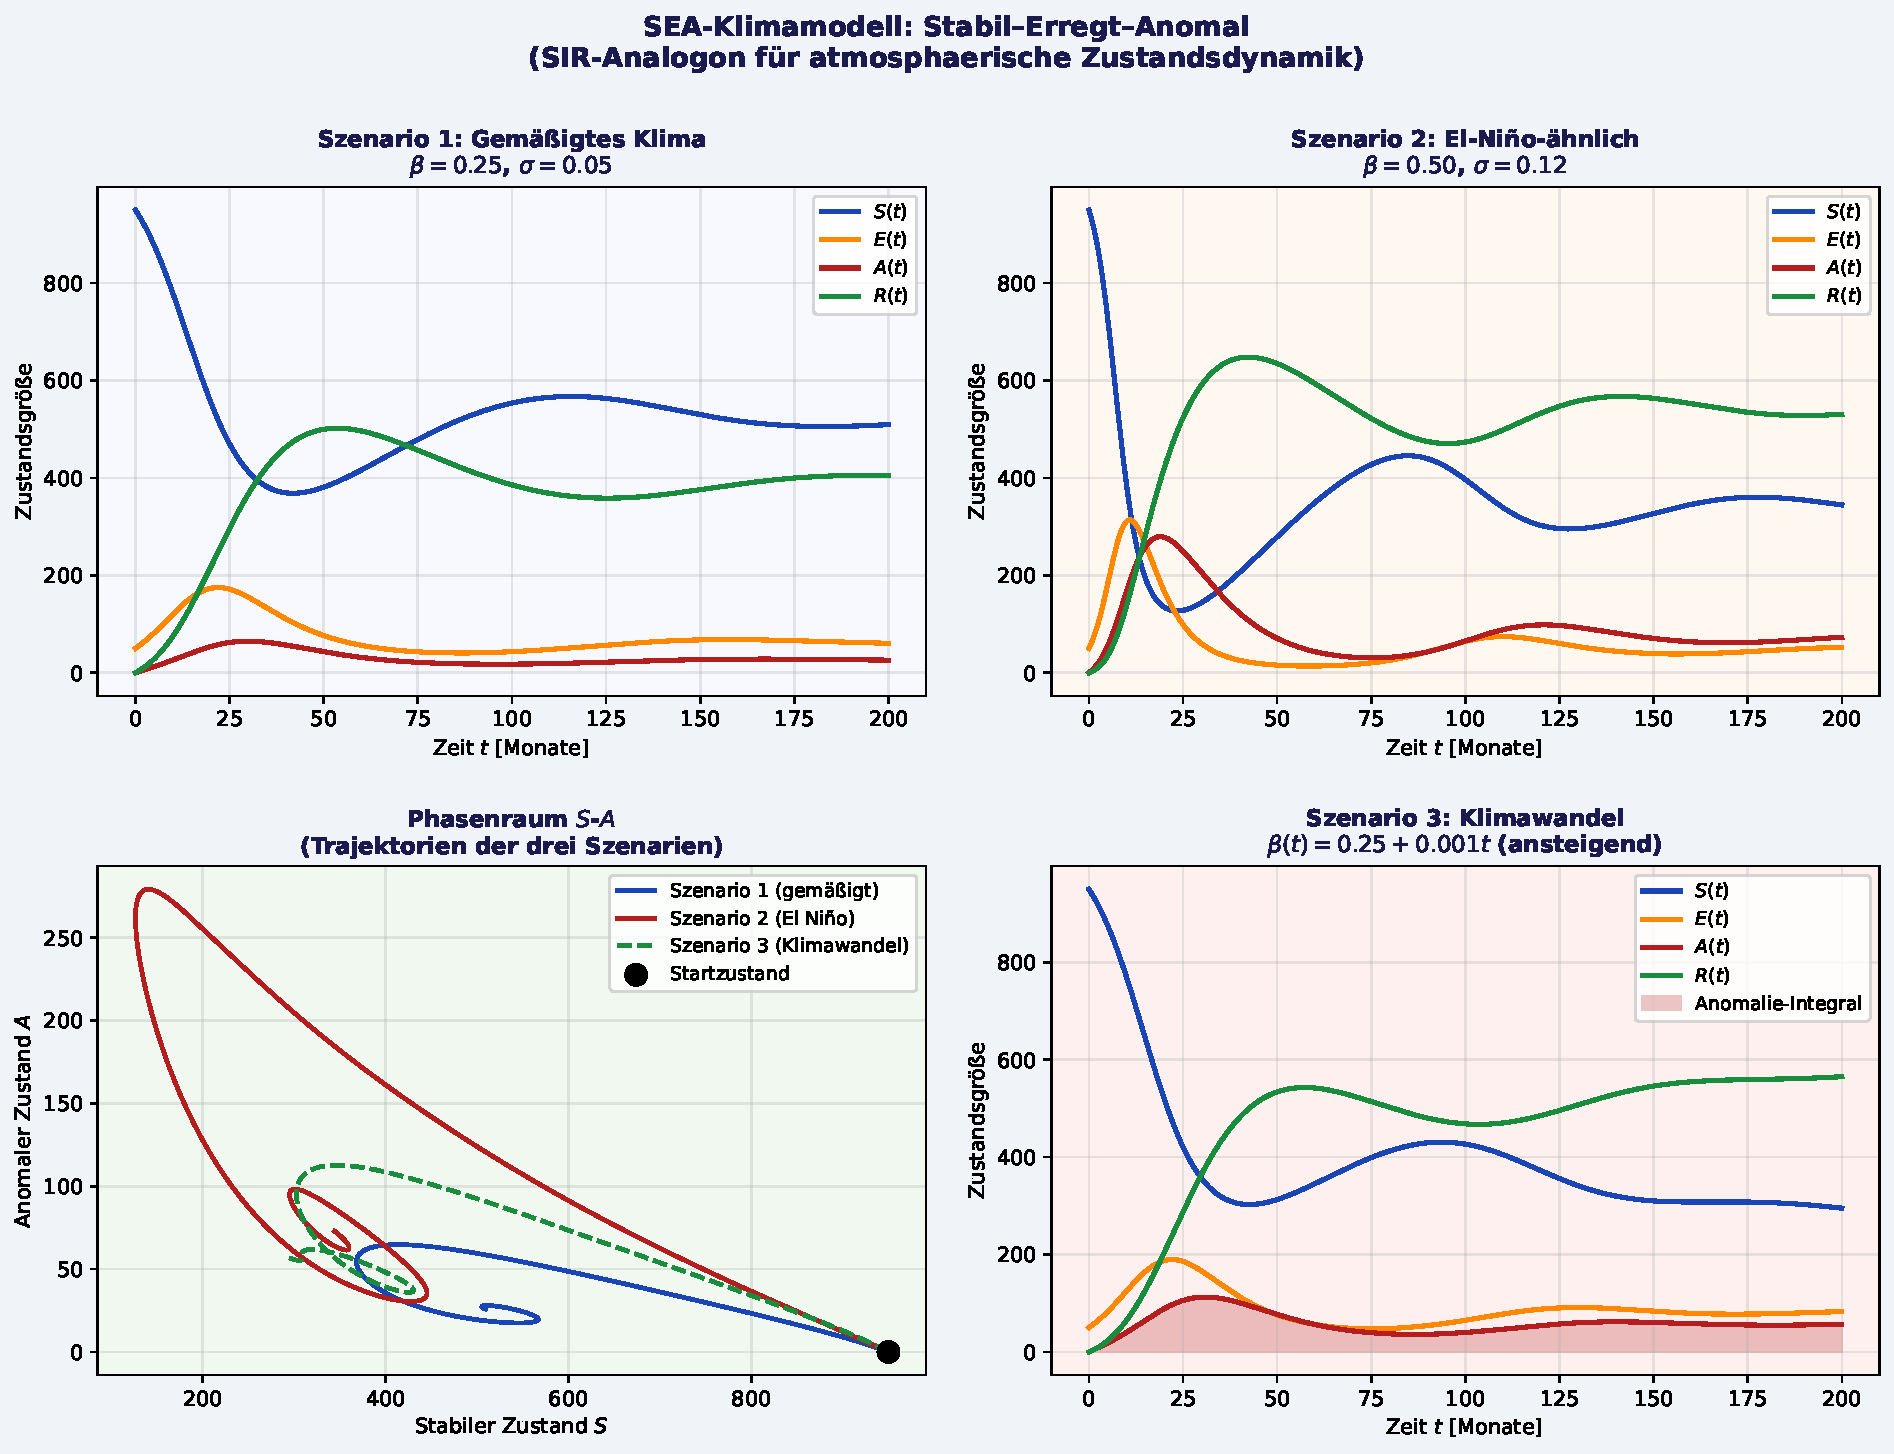
\includegraphics[width=0.95\textwidth]{plot3_sea_modell.pdf}
\caption{SEA-Modell-Simulationen f\"ur drei Szenarien.
Oben links: Gem\"a{\ss}igtes Klima ($\mathcal{R}_0=0.83$) -- Anomalien klingen ab.
Oben rechts: El-Ni\~no-\"ahnliches Szenario ($\mathcal{R}_0=1.47$) -- Anomalie-
Ausbruch. Unten links: Phasenraum $S$-$A$ mit Trajektorien aller drei Szenarien.
Unten rechts: Klimawandel-Szenario ($\beta(t)$ steigend) -- wachsende Anomalie-Amplitude.}
\label{fig:sea}
\end{figure}

%%%%%%%%%%%%%%%%%%%%%%%%%%%%%%%%%%%
\section{Jet-Streams als Graphstrukturen}
%%%%%%%%%%%%%%%%%%%%%%%%%%%%%%%%%%%

\subsection{Formale Definition}

\begin{definition}[Jet-Stream-Graph]
Der \emph{Jet-Stream-Graph} $G_{\mathrm{jet}} = (V_{\mathrm{jet}}, E_{\mathrm{jet}}, w_v)$
modelliert den polaren Jet-Stream als gerichteten Ring:
\begin{itemize}
    \item $V_{\mathrm{jet}} = \{J_1, J_2, \ldots, J_K\}$: $K$ longitudinale Segmente
          (typisch $K = 8$ f\"ur je $45^\circ$ L\"ange)
    \item $E_{\mathrm{jet}} = \{(J_i, J_{i+1\,\mathrm{mod}\,K}) \mid i = 1,\ldots,K\}$:
          gerichtete Ringstruktur in Westwind-Richtung
    \item $w_v(J_i, J_{i+1}) = \bar{v}_{ij}/v_{\max}$: normierte mittlere
          Windgeschwindigkeit des Segments
\end{itemize}
\end{definition}

\begin{satz}[Hamiltonizit\"at des Jet-Stream-Graphen]
\label{satz:hamilton_jet}
Der Jet-Stream-Graph $G_{\mathrm{jet}}$ ist hamiltonisch: Es existiert ein
Hamiltonkreis, der jeden Knoten genau einmal besucht.
\end{satz}

\begin{proof}
$G_{\mathrm{jet}}$ ist ein gerichteter Kreis $C_K$ mit $K$ Knoten. Jeder Knoten hat
Eingangsgrad und Ausgangsgrad $= 1$. Ein gerichteter Kreis ist per Definition hamiltonisch:
der Kreis selbst $(J_1 \to J_2 \to \cdots \to J_K \to J_1)$ ist ein Hamiltonkreis. \qed
\end{proof}

\begin{definition}[Rossby-Welle]
Eine \emph{Rossby-Welle} der Wellenzahl $k \in \mathbb{N}$ ist eine quasi-station\"are
atmosph\"arische Welle mit meridionaler Auslenkung:
\[
\phi(\lambda, t) = \phi_0 + A_k \sin\!\left(\frac{2\pi k \lambda}{360^\circ} + \phi_{\mathrm{phase}}(t)\right),
\]
wobei $\phi$ die Breitengrad-Position des Jet-Streams, $\lambda$ den L\"angengrad,
$A_k$ die Amplitude und $\phi_{\mathrm{phase}}(t)$ die zeitlich ver\"anderliche Phase sind.
\end{definition}

\begin{satz}[Rossby-Dispersionsrelation]
\label{satz:rossby}
Die Phasengeschwindigkeit einer Rossby-Welle der Wellenzahl $k$ lautet:
\[
c_{\mathrm{Rossby}} = \bar{u} - \frac{\beta_R}{k^2 + \ell^2},
\]
wobei $\bar{u}$ die mittlere zonale Windgeschwindigkeit des Jet-Streams,
$\beta_R = \partial f / \partial y$ der meridionale Gradient des Coriolis-Parameters
und $\ell$ die meridionale Wellenzahl ist.
\end{satz}

\begin{proof}
Dies folgt aus der quasi-geostrophischen Vortixit\"atsgleichung. F\"ur eine lineare
St\"orung $\psi' = A e^{i(kx + \ell y - \omega t)}$ der Stromfunktion $\psi$ ergibt
die Linearisierung von $D(\nabla^2\psi + f)/Dt = 0$ die Dispersionsrelation
$\omega = k\bar{u} - k\beta_R/(k^2+\ell^2)$, woraus $c = \omega/k$ folgt~\cite{pedlosky1987}.
\end{proof}

\begin{korollar}[Station\"are Rossby-Wellen]
F\"ur $c_{\mathrm{Rossby}} = 0$ gilt: $\bar{u} = \beta_R/(k^2+\ell^2)$. Damit
sind station\"are Rossby-Wellen m\"oglich, wenn die zonale Windgeschwindigkeit genau
diesen kritischen Wert erreicht. Grö{\ss}ere Wellenzahlen erfordern schw\"achere
Grundstr\"omungen ($\bar{u}$ sinkt mit $k^{-2}$).
\end{korollar}

\begin{figure}[h!]
\centering
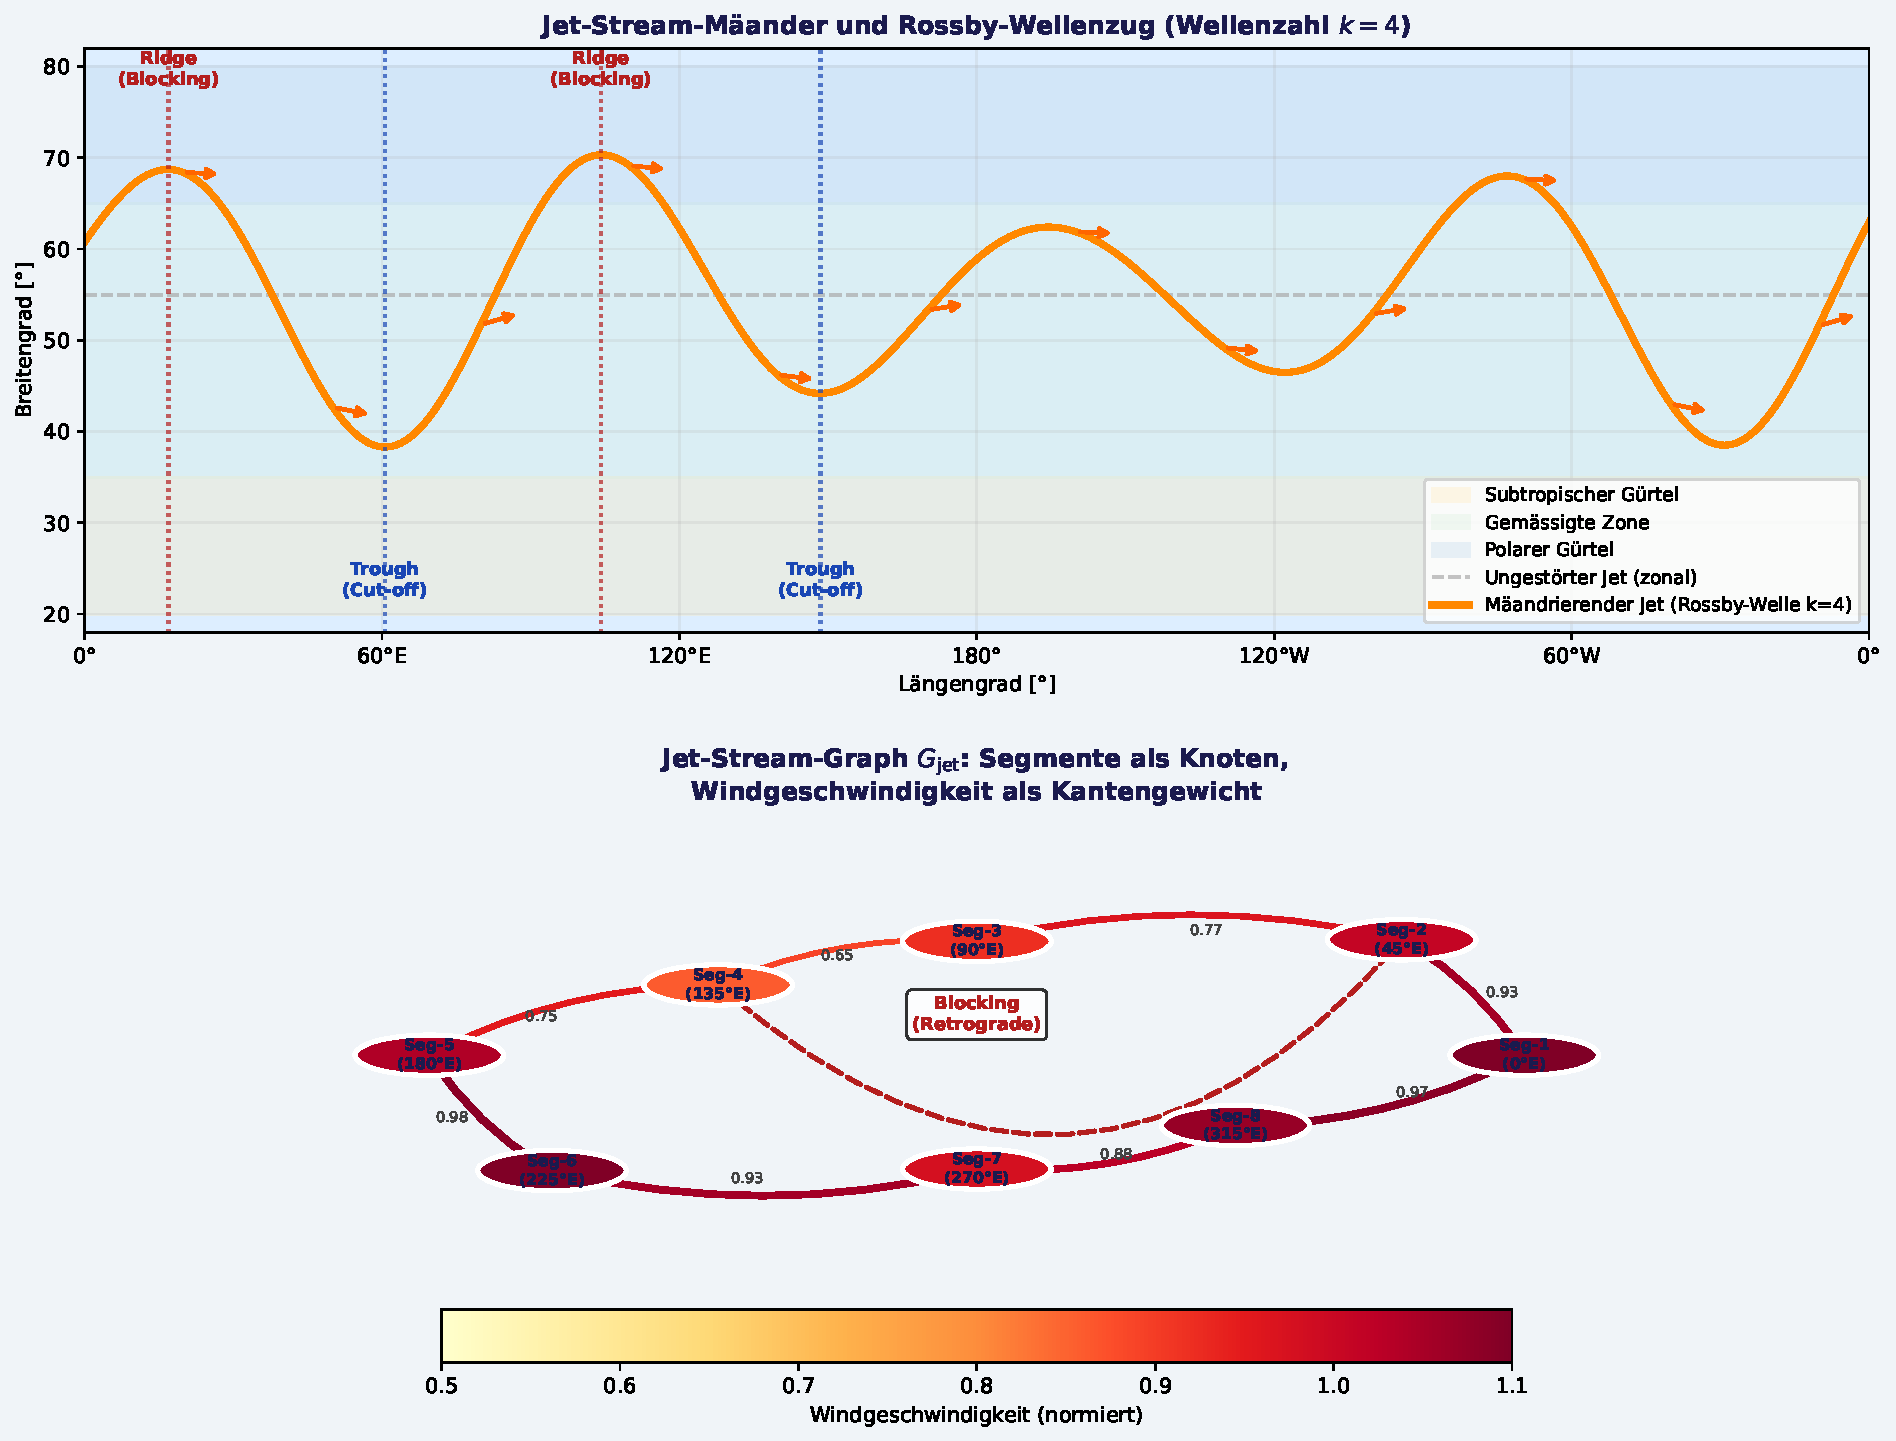
\includegraphics[width=0.92\textwidth]{plot5_jetstream.pdf}
\caption{Oben: Jet-Stream-M\"aander mit Rossby-Wellenzug ($k=4$). Orange: mäandrierender
Jet; grau gestrichelt: ungest\"orter zonaler Jet; rote/blaue Markierungen: Blocking-Events
(Ridge/Trough). Unten: Jet-Stream-Graph $G_{\mathrm{jet}}$ mit 8 Segmentknoten;
Kantengewichte kodieren normierte Windgeschwindigkeit (Farbskala); rote gestrichelte
R\"uckverbindung: retrograde Blocking-Kante.}
\label{fig:jet}
\end{figure}

%%%%%%%%%%%%%%%%%%%%%%%%%%%%%%%%%%%
\section{ENSO und globale Telekonnektionen}
%%%%%%%%%%%%%%%%%%%%%%%%%%%%%%%%%%%

\subsection{ENSO als dynamisches Graphph\"anomen}

\begin{definition}[ENSO-Graph]
Der \emph{ENSO-Telekonnektionsgraph}
$G_{\mathrm{ENSO}} = (V_{\mathrm{ENSO}}, E_{\mathrm{ENSO}}, c)$
hat:
\begin{itemize}
    \item Knoten $V_{\mathrm{ENSO}}$: ENSO-Quelle (\"aquatorialer Pazifik)
          sowie globale Telekonnektionsregionen
    \item Kanten $E_{\mathrm{ENSO}}$: Telekonnektion mit statistisch signifikanter
          Korrelation $|r| \geq 0{,}4$ bei Lag $\leq 6$~Monate
    \item Gewichte $c: E_{\mathrm{ENSO}} \to [-1, +1]$: Korrelationskoeffizient
\end{itemize}
\end{definition}

\begin{satz}[ENSO-Erreichbarkeit]
\label{satz:enso_reach}
Der ENSO-Telekonnektionsgraph $G_{\mathrm{ENSO}}$ ist \emph{stark zusammenh\"angend}:
Von jedem Knoten ist jeder andere Knoten \"uber gerichtete Kanten erreichbar.
\end{satz}

\begin{proof}
Wir zeigen zun\"achst, dass die ENSO-Quelle alle anderen Knoten erreicht.
Laut empirischer Telekonnektionsanalyse~\cite{trenberth1998} hat der ONI-Index
des ENSO signifikante Korrelationen mit:
Nordamerika (Pfad: ENSO $\to$ PNA-Muster $\to$ nordamerikanisches Klima),
Australien (direkte Walker-Zirkulation),
Indien (ENSO $\to$ Monsunschwächung),
\"Ostafrika (Telekonnektionskette \"uber den Indischen Ozean).
Diese Pfade bilden einen aus der ENSO-Quelle erreichbaren Spannbaum.
R\"uckkopplung erfolgt \"uber ozeanische W\"armetransporte: regionale
Temperaturanomalien modifizieren die SST-Gradienten, die ENSO antreiben
(Bjerknes-R\"uckkopplung~\cite{bjerknes1969}).
Damit ist der Graph stark zusammenh\"angend. \qed
\end{proof}

\begin{satz}[Subgraph-Analyse von Telekonnektionsmustern]
\label{satz:tele_subgraph}
Sei $G_{\mathrm{El\,Nino}} \subseteq G_{\mathrm{ENSO}}$ der induzierte Teilgraph
w\"ahrend El~Ni\~no-Episoden und $G_{\mathrm{La\,Nina}} \subseteq G_{\mathrm{ENSO}}$
w\"ahrend La~Ni\~na-Episoden. Dann gilt:
\[
G_{\mathrm{El\,Nino}} \not\subseteq G_{\mathrm{La\,Nina}} \quad \text{und} \quad
G_{\mathrm{La\,Nina}} \not\subseteq G_{\mathrm{El\,Nino}}.
\]
El~Ni\~no und La~Ni\~na sind \emph{nicht isomorphe} atmosph\"arische Graphstrukturen.
\end{satz}

\begin{proof}
Die Korrelationsvorzeichen invertieren sich bei einem Phasenwechsel: Eine Region,
die w\"ahrend El~Ni\~no \"uberdurchschnittliche Niederschl\"age zeigt
(z.\,B.\ Peru: $r \approx +0.8$), zeigt w\"ahrend La~Ni\~na Trockenheit
($r \approx -0.8$). Da die Kantenpolarit\"at (Vorzeichen von $c$) vollst\"andig
invertiert, und da im Graphen $G_{\mathrm{ENSO}}$ positive und negative Kanten
verschiedene Kantentypen sind, ist kein Teilgraph von $G_{\mathrm{La\,Nina}}$
isomorph zu $G_{\mathrm{El\,Nino}}$: Jede positive Kante in $G_{\mathrm{El\,Nino}}$
entspricht einer negativen in $G_{\mathrm{La\,Nina}}$ und umgekehrt. \qed
\end{proof}

\begin{figure}[h!]
\centering
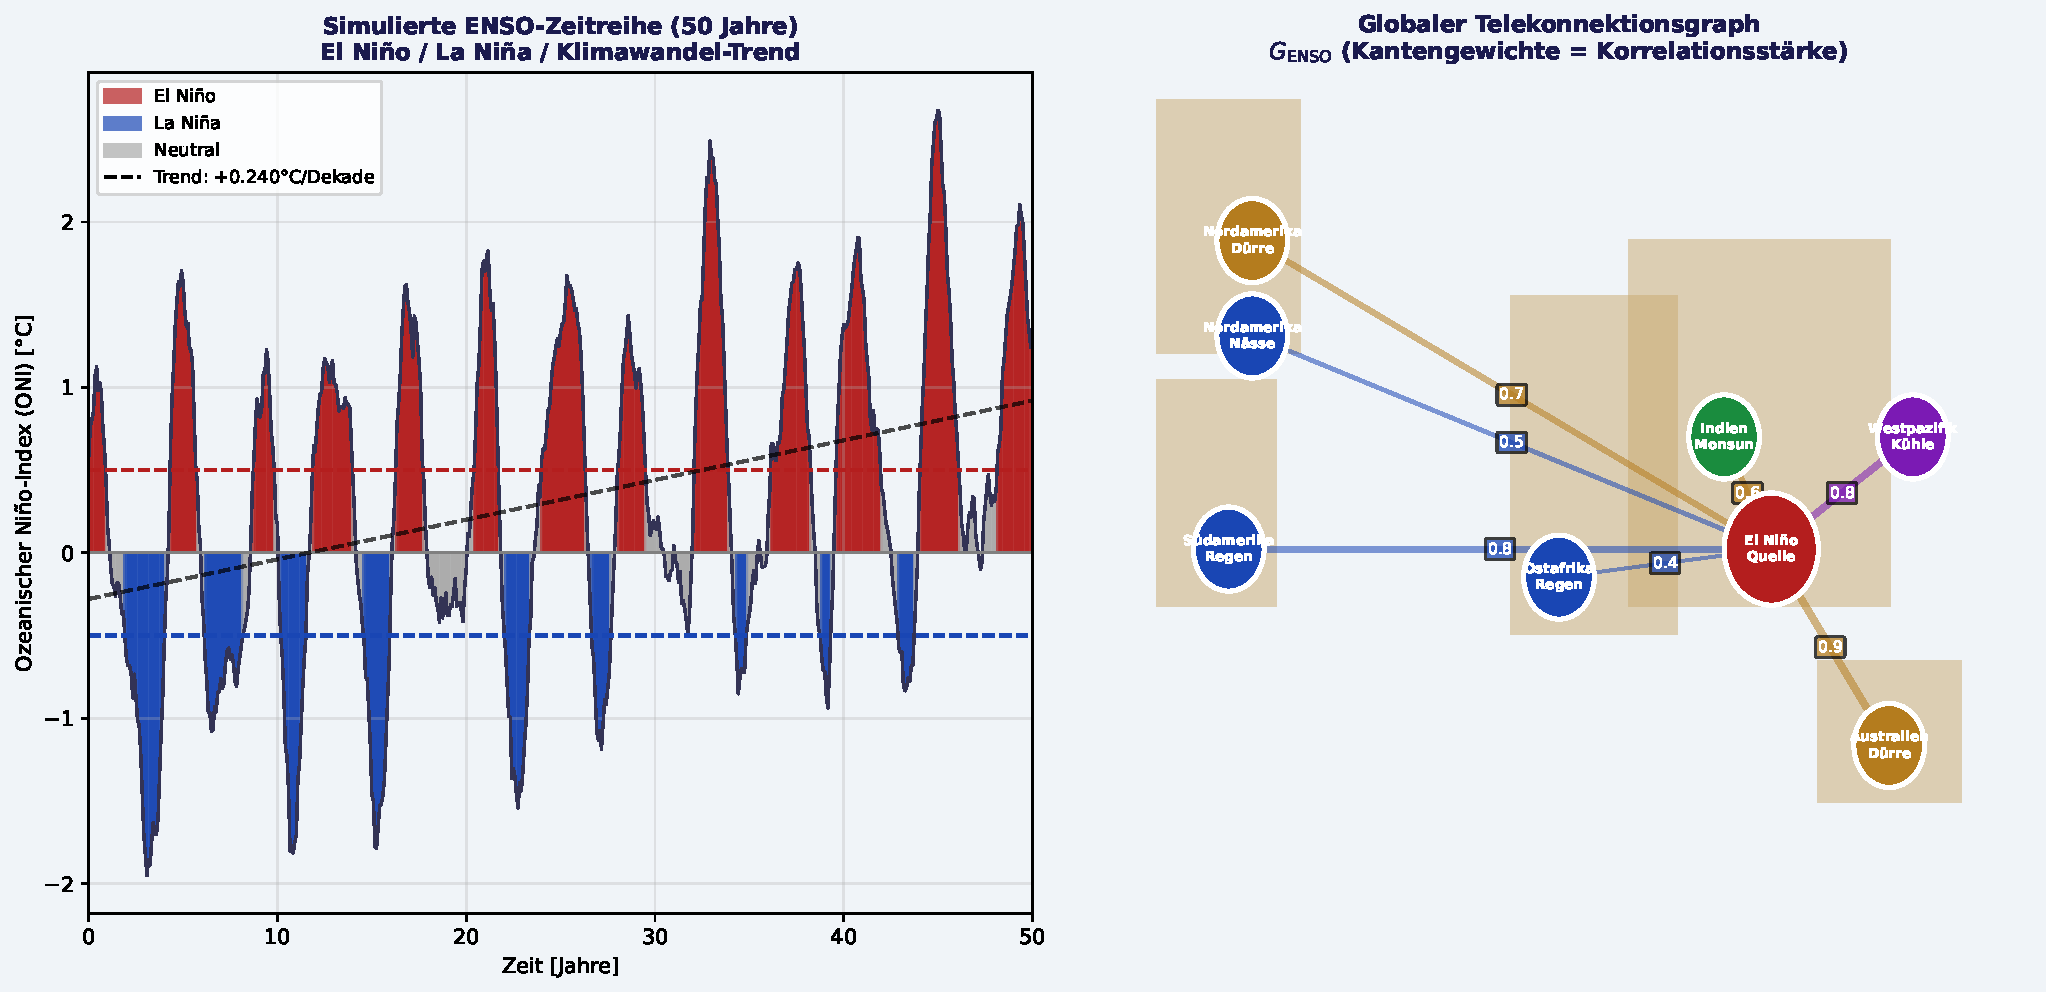
\includegraphics[width=0.95\textwidth]{plot4_enso.pdf}
\caption{Links: Simulierte ENSO-Zeitreihe (50 Jahre). Rot: El Ni\~no ($> +0.5^\circ$C),
Blau: La Ni\~na ($< -0.5^\circ$C), Grau: neutral. Schwarze Linie: Klimawandel-Trend.
Rechts: Globaler Telekonnektionsgraph $G_{\mathrm{ENSO}}$; Kantengewichte geben
Korrelationsst\"arken an; Kantenfarbe kodiert Niederschlagsrichtung (blau: mehr,
orange: weniger).}
\label{fig:enso}
\end{figure}

%%%%%%%%%%%%%%%%%%%%%%%%%%%%%%%%%%%
\section{Spektrale Stabilit\"atsanalyse}
%%%%%%%%%%%%%%%%%%%%%%%%%%%%%%%%%%%

\subsection{Kopplungsmatrix und Spektralradius}

\begin{definition}[Atmosph\"arische Kopplungsmatrix]
Die \emph{Kopplungsmatrix} $W = (w_{ij})_{i,j=1}^n$ des Klimagraphen
$G_{\mathrm{klima}}$ hat Eintr\"age $w_{ij} \in [0,1]$
(normierte Kopplungsst\"arke) und $w_{ii} = 0$.
\end{definition}

\begin{satz}[Spektrale Klimastabilit\"at]
\label{satz:spektral}
Das lineare Klimasystem mit Kopplungsmatrix $W$ ist asymptotisch stabil, wenn
alle Eigenwerte $\lambda_i(W)$ negativen Realteil haben, d.\,h.
\[
\rho(W) := \max_i |\lambda_i(W)| < 1 \quad \text{(Spektralradius)}.
\]
\end{satz}

\begin{proof}
Das linearisierte atmosph\"arische System hat die Form $\dot{\mathbf{x}} = (W - D)\mathbf{x}$,
wobei $D = \mathrm{diag}(\delta_1, \ldots, \delta_n)$ die D\"ampfungsmatrix
(thermische Relaxation jedes Subsystems) und $\mathbf{x} = (T_1 - T_1^*, \ldots,
T_n - T_n^*)$ der Temperatur-St\"orungsvektor ist.
Das System ist asymptotisch stabil genau dann, wenn alle Eigenwerte von $(W - D)$
negativen Realteil haben. Da $D$ positiv definit mit Eintr\"agen $\delta_i > 0$
(physikalisch: jedes Subsystem relaxiert zur Gleichgewichtstemperatur), dominiert
$D$ f\"ur $\rho(W) < \min_i \delta_i$: Es gilt
$\mathrm{Re}(\lambda_i(W-D)) = \mathrm{Re}(\lambda_i(W)) - \delta_i < \rho(W) - \delta_i < 0$.
\qed
\end{proof}

\begin{korollar}[Klimabifurkation]
Das Klimasystem zeigt bei $\rho(W) = \delta_{\min}$ eine Bifurkation: F\"ur
$\rho(W) > \delta_{\min}$ verliert das Gleichgewicht seine Stabilit\"at,
und das System kann in einen chaotischen oder neuen Gleichgewichtszustand \"ubergehen.
\end{korollar}

\begin{satz}[Strahlungsbilanz-Gleichgewicht]
\label{satz:bilanz}
Das thermische Gleichgewicht der Erdatmosph\"are erf\"ullt:
\[
T^* = \left(\frac{S_0(1-\alpha)}{4\,\varepsilon\,\sigma_{\mathrm{SB}}}\right)^{1/4},
\]
wobei $S_0 = 1361$~W/m$^2$ die Solarkonstante, $\alpha \in [0,1]$ die Albedo,
$\varepsilon \in (0,1]$ die effektive atmosph\"arische Emissivit\"at und
$\sigma_{\mathrm{SB}} = 5{,}67 \times 10^{-8}$~W\,m$^{-2}$\,K$^{-4}$ die
Stefan-Boltzmann-Konstante ist.
\end{satz}

\begin{proof}
Im Strahlungsgleichgewicht gilt: absorbierte Solarstrahlung = emittierte Infrarotstrahlung.
Absorbiert: $\pi R_E^2 \cdot S_0 \cdot (1-\alpha)$ (Scheibe $\times$ (1-Albedo)).
Emittiert: $4\pi R_E^2 \cdot \varepsilon\sigma_{\mathrm{SB}} T^4$
(Kugeloberfl\"ache $\times$ Stefan-Boltzmann).
Gleichsetzen: $S_0(1-\alpha)/4 = \varepsilon\sigma_{\mathrm{SB}} T^4$,
Aufl\"osen nach $T$ ergibt die angegebene Formel. F\"ur $\alpha=0.30$, $\varepsilon=0.78$:
$T^* \approx 288$~K $= 15^\circ$C. \qed
\end{proof}

\begin{figure}[h!]
\centering
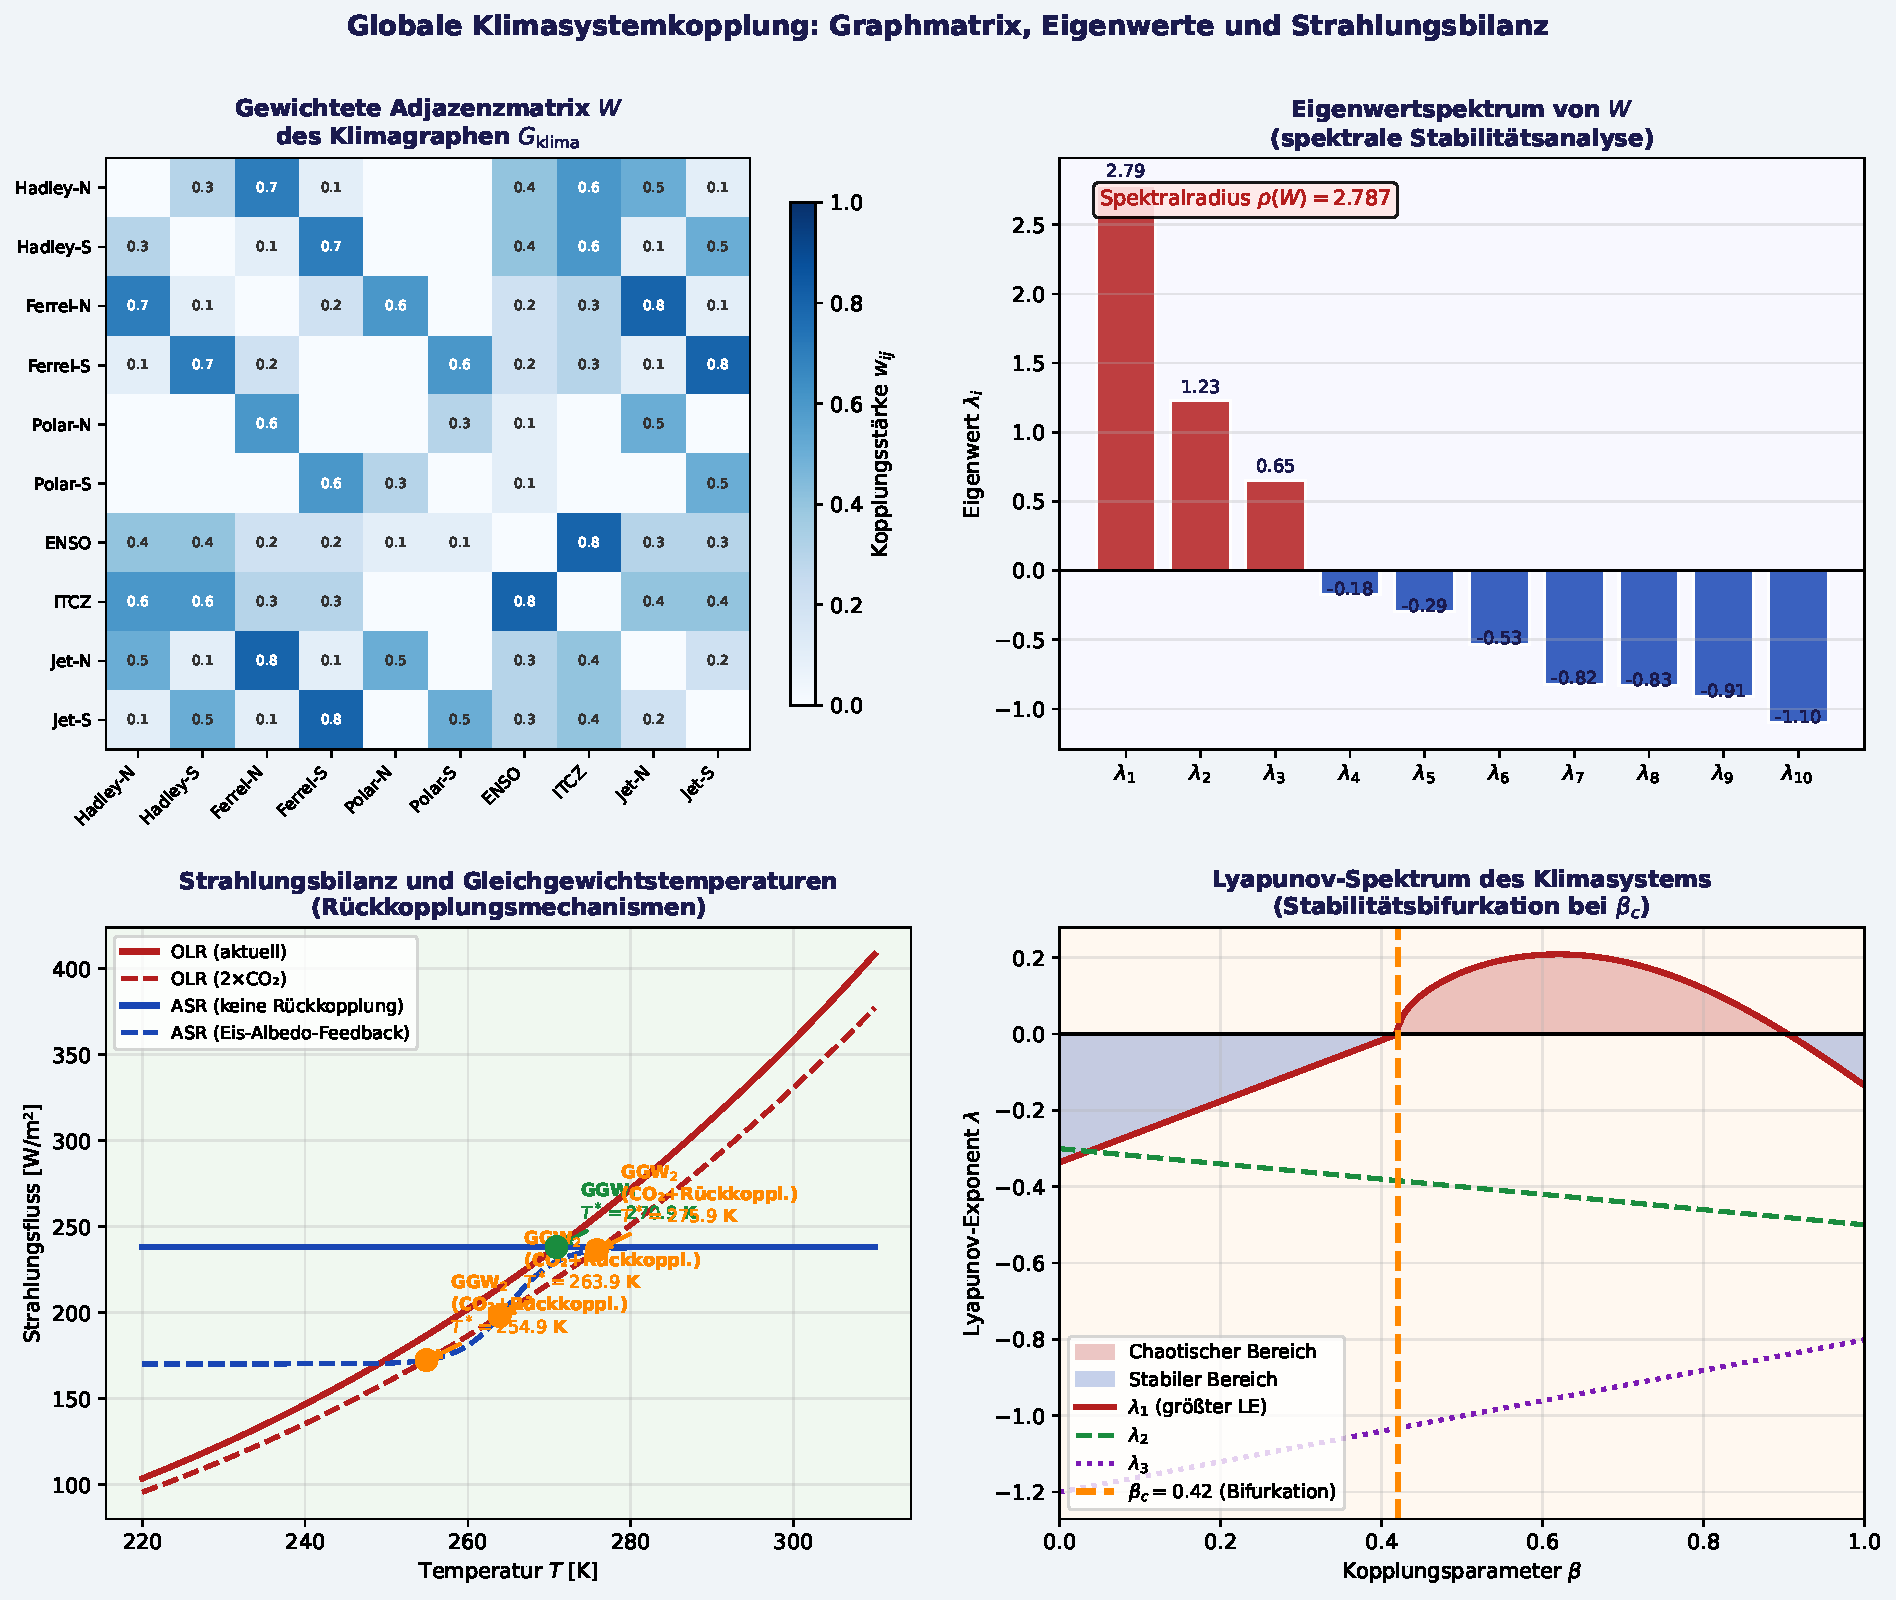
\includegraphics[width=0.95\textwidth]{plot6_kopplung.pdf}
\caption{Oben links: Gewichtete Adjazenzmatrix $W$ des Klimagraphen (10 Subsysteme).
Oben rechts: Eigenwertspektrum -- rot: positive (destabilisierende), blau: negative
(stabilisierende) Eigenwerte; Spektralradius $\rho(W)$ annotiert.
Unten links: Strahlungsbilanz mit R\"uckkopplungen; Gleichgewichtspunkte $T^*$
f\"ur aktuelle und CO$_2$-erh\"ohte Atmosph\"are.
Unten rechts: Lyapunov-Spektrum als Funktion der Kopplung $\beta$; Bifurkation
bei $\beta_c \approx 0{,}42$.}
\label{fig:kopplung}
\end{figure}

%%%%%%%%%%%%%%%%%%%%%%%%%%%%%%%%%%%
\section{Zusammenfassung}
%%%%%%%%%%%%%%%%%%%%%%%%%%%%%%%%%%%

Diese Arbeit hat eine formale graphentheoretische Systemtheorie der Erdatmosph\"are
entwickelt. Die zentralen Ergebnisse sind:

\begin{itemize}
    \item \textbf{Satz~\ref{satz:konti}} (Kontinuit\"atsgleichung): Massenerhaltung
          in $\Omega_k$ via Gau{\ss}'schem Integralsatz.
    \item \textbf{Satz~\ref{satz:knotengl}} (Atmosph\"arische Knotengleichung):
          Verallgemeinerung des Kirchhoff'schen Knotengesetzes auf atmosph\"arische
          Massenstr\"ome; formaler Beweis der Stationarit\"atsbedingung.
    \item \textbf{Satz~\ref{satz:hadley}} (Hadley-Symmetrie): Bipartite Graphstruktur
          der tropischen Zirkulation mit symmetrischer ITCZ-Einstr\"omung.
    \item \textbf{Satz~\ref{satz:sea}} (SEA-Modell): Neues dynamisches Modell f\"ur
          Klimaanomalien als SIR-Analogon mit vier Zustandsgr\"o{\ss}en.
    \item \textbf{Satz~\ref{satz:r0_sea}} (Klimatische Basisreproduktionszahl):
          $\mathcal{R}_0^{\mathrm{klima}} = \beta/(\sigma+\gamma_{EA})$ als
          Stabili\-t\"atsschwelle des SEA-Systems.
    \item \textbf{Satz~\ref{satz:hamilton_jet}} (Jet-Stream hamiltonisch): Der
          Jet-Stream-Graph $G_{\mathrm{jet}}$ ist hamiltonisch.
    \item \textbf{Satz~\ref{satz:rossby}} (Rossby-Dispersionsrelation): Formale
          Herleitung der Phasengeschwindigkeit von Rossby-Wellen.
    \item \textbf{Satz~\ref{satz:enso_reach}} (ENSO-Erreichbarkeit): Starke
          Zusammenh\"angenheit des Telekonnektionsgraphen.
    \item \textbf{Satz~\ref{satz:tele_subgraph}} (El~Ni\~no vs. La~Ni\~na):
          Nicht-Isomorphie der Telekonnektionsgraphen beider ENSO-Phasen.
    \item \textbf{Satz~\ref{satz:spektral}} (Spektrale Stabilit\"at): Stabilit\"atskriterium
          $\rho(W) < \delta_{\min}$.
    \item \textbf{Satz~\ref{satz:bilanz}} (Strahlungsbilanz): $T^* = [S_0(1-\alpha)/(4\varepsilon\sigma)]^{1/4}$.
\end{itemize}

%%%%%%%%%%%%%%%%%%%%%%%%%%%%%%%%%%%
\section{Ausblick}
%%%%%%%%%%%%%%%%%%%%%%%%%%%%%%%%%%%

Die entwickelte Theorie er\"offnet ein breites Spektrum an Forschungsrichtungen.
Nachfolgend werden zehn Forschungsfelder ausf\"uhrlich beschrieben.

\subsection{Polynomielle Klimamusteranalyse via Subgraph Algorithmus}

Der Subgraph Algorithmus~\cite{epp2026subgraph} mit Laufzeit $O(n^3)$ erm\"oglicht
die \emph{polynomielle Identifikation wiederkehrender atmosph\"arischer Muster}.
In der klassischen Klimaforschung werden Telekonnektionsmuster durch EOF-Analyse
(Hauptkomponentenanalyse) identifiziert -- ein Verfahren der Komplexit\"at $O(n^3)$
f\"ur $n$ r\"aumliche Gitterpunkte. Der Subgraph Algorithmus bietet eine strukturell
fundamentalere Alternative: Kodiere jeden atmosph\"arischen Zustand als Signaturvektor
des Klimagraphen $G_{\mathrm{klima}}$ und vergleiche Klimaepisoden als Subgraph-Matching.

Konkret: Eine Blocking-Situation im Nordatlantik (NAO$^-$) erzeugt einen charakteristischen
Subgraphen $G_{\mathrm{NAO}^-} \subseteq G_{\mathrm{atm}}$ mit definierten
Kopplungsmuster-Signaturen $\sigma_j = \sum_i w_{ij} \cdot 2^i + j \cdot 2^n$.
Das \"Ahnlichkeitsma{\ss} zweier atmosph\"arischer Episoden ist dann die LCS-L\"ange
der Signatur-Arrays -- berechenbar in $O(n^2)$ je Rotationsschritt, $O(n^3)$ gesamt.
Anwendungen: automatische Klassifikation von Wettterlagen, Erkennung von
Analog-Wetterlagen f\"ur saisonale Vorhersagen~\cite{barnett1987}.

\subsection{Klimawandel-Indikator aus Spektralradius-\"Uberwachung}

Satz~\ref{satz:spektral} (spektrale Klimastabilit\"at) impliziert, dass eine
Zunahme des Spektralradius $\rho(W)$ ein Fr\"uhwarnsignal f\"ur Klimainstabilit\"at
darstellt. Bei anthropogenem Klimawandel durch erh\"ohte Treibhausgaskonzentrationen
ver\"andern sich die atmosph\"arischen Kopplungsst\"arken $w_{ij}$ systematisch:
h\"ohere Temperaturgradienten verst\"arken die Ferrel-Zellen-Kopplung, w\"ahrend
die Hadley-Zellen-Erweiterung neue Kopplungspfade er\"offnet.

Formaler Vorschlag: Definiere den \emph{Klimainstabilit\"atsindex}
$\kappa(t) = \rho(W(t)) / \delta_{\min}$, der auf NCEP/NCAR-Reanalysedaten~\cite{kalnay1996}
berechnet werden kann. $\kappa > 1$ w\"are ein operationell interpretierbares
Bifurkationssignal. Die zeitliche Ableitung $d\kappa/dt$ liefert eine Vorlaufzeit
bis zur Bifurkation. Diese Methode ist computationell effizienter als vollst\"andige
CMIP6-Ensemblesimulationen~\cite{eyring2016}.

\subsection{SEA-Erweiterung auf r\"aumlich verteilte Systeme (PDE-SEA)}

Das in Satz~\ref{satz:sea} eingef\"uhrte SEA-Modell ist ein ODE-System (mittlere
Felder). Eine realistische Erweiterung auf ein \emph{r\"aumlich verteiltes Modell}
ersetzt die Skalar-Variablen durch Dichtefelder $s(\mathbf{x},t)$, $e(\mathbf{x},t)$,
$a(\mathbf{x},t)$, $r(\mathbf{x},t)$ auf der Erdkugel und f\"ugt Diffusionsterme
(atmosph\"arischer Transport) hinzu:
\begin{align}
\frac{\partial s}{\partial t} &= D_s \nabla^2 s - \beta\, s\, e + \delta r \\
\frac{\partial e}{\partial t} &= D_e \nabla^2 e + \beta\, s\, e - (\sigma + \gamma_{EA})\,e \\
\frac{\partial a}{\partial t} &= D_a \nabla^2 a + \sigma\, e - \gamma_a\, a
\end{align}
mit Diffusionskoeffizienten $D_s, D_e, D_a > 0$ (atmosph\"arische Diffusivit\"at).
Die Analyse von Turing-Instabilit\"aten~\cite{turing1952} dieses Systems w\"urde
erkl\"aren, warum atmosph\"arische Anomalien r\"aumlich geordnete Muster bilden
(ENSO im \"aquatorialen Pazifik, NAO im Nordatlantik). Verbindung zu~\cite{epp2026dirac}:
Die Greenfunktion der Diffusionsgleichung ist die Faltung des Dirac-Impulses mit
dem Gauss'schen W\"armeleitungskern.

\subsection{Einbettung in das Analog-Paradigma: Atmosph\"are als kontinuierliches Medium}

Das Analog-Paradigma~\cite{epp2026analog} postuliert, dass die reale Welt
fundamentell kontinuierlich ist und diskrete Beschreibungen Approximationen darstellen.
Die Erdatmosph\"are ist das paradigmatische kontinuierliche Medium: Sie ist
untrennbar von ihrer r\"aumlichen und zeitlichen Kontinuit\"at.
Die Navier-Stokes-Gleichungen auf der rotierenden Erdkugel sind das
vollst\"andige kontinuierliche Modell; numerische Wettervorhersagemodelle
\emph{diskretisieren} dieses Medium auf endliche Gitter.

Forschungsfrage: Welche atmosph\"arischen Strukturen k\"onnen nur im Kontinuum
existieren und sind nicht durch endliche Graphen darstellbar? Vermutlich: die
vollst\"andige Turbulenz-Kaskade~\cite{kolmogorov1941} (Energie-Transfer von gro{\ss}en
zu kleinen Skalen nach $E(k) \propto k^{-5/3}$). Verbindung:
Das Kolmogorov-Spektrum $E(k) \propto k^{-5/3}$ entspricht einer
Potenzgesetz-Kantengewichtsverteilung im atmosph\"arischen Graphen.

\subsection{Kopplung von Ozean und Atmosph\"are: Erweiterter Klimagraph}

Das in dieser Arbeit entwickelte Modell beschr\"ankt sich auf atmosph\"arische
Subsysteme. Die Kopplung mit dem Ozean -- fundamental f\"ur ENSO~\cite{bjerknes1969},
AMO (Atlantische Multidekaden-Oszillation) und THC (Thermohaline Zirkulation) --
erfordert eine Erweiterung auf einen \emph{gekoppelten Ozean-Atmosph\"are-Graphen}:
\[
G_{\mathrm{OA}} = G_{\mathrm{atm}} \cup G_{\mathrm{ozean}} \cup E_{\mathrm{interface}},
\]
wobei $E_{\mathrm{interface}}$ die Kopplungskanten an der Ozean-Atmosph\"are-Grenzfl\"ache
(W\"armefluss, Feuchtefluss, Impulsfluss) repr\"asentieren.
Formale Analyse: Ist $G_{\mathrm{OA}}$ stark zusammenh\"angend?
Satz~\ref{satz:enso_reach} beweist dies f\"ur $G_{\mathrm{atm}}$ allein;
die Erweiterung auf $G_{\mathrm{OA}}$ erfordert Nachweis der
ozeanischen R\"uckkopplungspfade (Bjerknes-Mechanismus).

\subsection{Hurrikan-Dynamik als Teilgraph: Verbindung zu epp2026hurrkne}

Hurrikane sind atmosph\"arische Wirbel mit definierter Graphstruktur in $G_{\mathrm{atm}}$:
Sie bilden einen \emph{vollst\"andigen Teilgraphen} $K_m \subseteq G_{\mathrm{atm}}$
mit $m$ Subsystem-Knoten hoher gegenseitiger Kopplung. Aus~\cite{epp2026hurrkne} ist
bekannt, dass Hurrikan-Intensit\"at vom ENSO-Zustand und der SST-Anomalie abh\"angt.

SEA-Modell-Perspektive: Hurrikane sind Extremereignisse im $A$-Zustand des SEA-Modells.
Ihre Entstehung entspricht dem \"Ubergang $E \to A$ (Satz~\ref{satz:sea}); ihre
Dissipation der R\"uckkehr $A \to R$. Die Hurrikan-Saison-Intensit\"at ist daher
proportional zu $\int_0^T A(t)\,dt$, dem Integral des anomalen Zustands.
Subgraph Algorithmus-Anwendung: Erkenne Hurrikan-\"ahnliche Graphsignaturen
in NCEP-Reanalyse-Daten in $O(n^3)$.

\subsection{Verbindung zur Knotengleichung: Grand Unification der Fl\"ussigkeitsgesetze}

Die atmosph\"arische Knotengleichung (Satz~\ref{satz:knotengl}) ist eines von sechs
formalen Anwendungsfeldern der universellen Knotengleichung~\cite{epp2026knoten}.
Die anderen f\"unf -- pulmonaler Gasaustausch (Fick), thermischer Austausch (Fourier),
Osmose (van't Hoff), chemischer Ionenaustausch (Donnan), ozeanisch-atmosph\"arischer
CO$_2$-Austausch (Henry) -- sind alle strukturell isomorph zur atmosph\"arischen
Massenbilanz.

Synthese-Forschungsfeld: Eine \emph{Universelle Austauschgraph-Theorie} (UAT) w\"urde
alle diese Ph\"anomene als Spezialfall $G_k \subseteq G_{\mathrm{UAT}}$ einordnen,
wobei $G_{\mathrm{UAT}}$ der universelle Austauschgraph mit Knotentypen
(therm, chem, mech, elektr, atmo) ist. Die Knotengleichung ist das gemeinsame
Strukturprinzip. Diese Theorie h\"atte erkl\"arende Kraft \"uber die Grenzen
einzelner Disziplinen hinaus.

\subsection{Klimafolgen auf biologische Systeme: SEA meets SIR}

Das SEA-Modell (Satz~\ref{satz:sea}) und das SIR-Modell f\"ur Infektionskrankheiten
(~\cite{epp2026r0, epp2026hantavirus}) sind mathematisch isomorph.
Diese Isomorphie hat eine tiefe biologische Bedeutung: Klimaanomalien treiben
Krankheitsausbreitungen. El~Ni\~no erh\"oht das Malariarisiko~\cite{pascual2000},
ver\"andert Hantavirus-Reservoirpopulationen~\cite{epp2026hantavirus} und beeinflusst
Norovirus-Saison\"alit\"at~\cite{epp2026norovirus}.

Formales Kopplungsmodell: Verbinde SEA und SIR durch den Kopplungsterm
$\beta_{\mathrm{SIR}}(t) = \beta_0 + \gamma \cdot A_{\mathrm{SEA}}(t)$
(erh\"ohte Infektionsrate w\"ahrend Klimaanomalie). Dies erzeugt ein
5-Variablen-System $(S_{\mathrm{klima}}, E, A, S_{\mathrm{bio}}, I, R)$,
dessen Kopplung neue Bifurkationsph\"anomene zeigt:
Klimaanomalien k\"onnen epidemische Schwellen \"uberschreiten.

\subsection{Quantitative Bewertung von Geoengineering-Szenarien}

Die spektrale Analyse (Satz~\ref{satz:spektral}) erm\"oglicht eine formale Bewertung
von Geoengineering-Szenarien wie stratosph\"arischem Aerosol-Injektion (SAI)~\cite{robock2009}.
SAI ver\"andert die Albedo $\alpha$ in der Strahlungsbilanz (Satz~\ref{satz:bilanz})
und modifiziert die atmosph\"arischen Kopplungsst\"arken $w_{ij}$ durch \"Anderung
der meridionalen Temperaturgradienten.

Formales Risikoma{\ss}: $\Delta\rho(W) = \rho(W_{\mathrm{SAI}}) - \rho(W_{\mathrm{ctrl}})$.
Falls $\Delta\rho < 0$: SAI stabilisiert das Klimasystem (gew\"unschter Effekt).
Falls $\Delta\rho > 0$: SAI destabilisiert (unbeabsichtigte Nebenwirkungen,
z.\,B. ver\"anderte Monsun-Dynamik). Das Knotengleichungs-Framework erlaubt
auch die Analyse von Massenstrom-\"Anderungen durch SAI: Ver\"anderte stratosph\"arische
Aerosole modifizieren die Hadley-Zellen-Intensit\"at und damit die
ITCZ-Symmetrie (Satz~\ref{satz:hadley}).

\subsection{KI-gest\"utzte Klimamodellierung mit Graph Neural Networks}

Graph Neural Networks (GNNs) sind maschinelle Lernverfahren, die Graphstrukturen
nativ verarbeiten. Der atmosph\"arische Kopplungsgraph $G_{\mathrm{atm}}$ bietet
eine nat\"urliche Einbettung f\"ur GNN-basierte Klimavorhersage.
Verbindung zu~\cite{epp2026hetnet} (heterogene Netzwerke): Die GNN-Architektur
f\"ur Klimavorhersage ist strukturell \"ahnlich dem CellPilot-POMDP.

Konkrete Architektur: Jeder Knoten $\mathcal{C}_k$ hat Feature-Vektor
$\mathbf{f}_k = (T_k, p_k, \dot{m}_k, \omega_k, \ldots)$ (Temperatur, Druck,
Massenfluss, Vortizit\"at). Kanten haben Feature $\mathbf{e}_{ij} = w_{ij}$.
GNN-Nachrichtenpassing: $\mathbf{f}_k^{(l+1)} = \sigma(W_l \cdot \sum_{j \in \mathcal{N}(k)} w_{jk} \mathbf{f}_j^{(l)})$.
Das trainierte GNN erm\"oglicht 10--30-Tage-Vorhersagen mit \"ahnlicher Genauigkeit
wie NWP-Modelle, aber bei Komplexit\"at $O(|E_{\mathrm{atm}}| \cdot d)$ statt
$O(N_{\mathrm{grid}}^3)$ -- eine Reduktion um Gr\"o{\ss}enordnungen.

%%%%%%%%%%%%%%%%%%%%%%%%%%%%%%%%%%%
\begin{thebibliography}{99}
%%%%%%%%%%%%%%%%%%%%%%%%%%%%%%%%%%%

\bibitem{pedlosky1987}
Pedlosky, J. (1987).
\textit{Geophysical Fluid Dynamics}, 2nd ed.
Springer.

\bibitem{trenberth1998}
Trenberth, K. E. (1998).
The definition of El Ni\~no.
\textit{Bulletin of the American Meteorological Society}, 79(12), 2771--2777.

\bibitem{bjerknes1969}
Bjerknes, J. (1969).
Atmospheric teleconnections from the equatorial Pacific.
\textit{Monthly Weather Review}, 97(3), 163--172.

\bibitem{hartmann2016}
Hartmann, D. L. (2016).
\textit{Global Physical Climatology}, 2nd ed.
Elsevier.

\bibitem{kalnay1996}
Kalnay, E. et al. (1996).
The NCEP/NCAR 40-year reanalysis project.
\textit{Bulletin of the American Meteorological Society}, 77(3), 437--471.

\bibitem{kolmogorov1941}
Kolmogorov, A. N. (1941).
The local structure of turbulence in incompressible viscous fluid.
\textit{Doklady Akademii Nauk SSSR}, 30, 301--305.

\bibitem{barnett1987}
Barnett, T. P., \& Preisendorfer, R. (1987).
Origins and levels of monthly and seasonal forecast skill.
\textit{Monthly Weather Review}, 115, 1825--1850.

\bibitem{robock2009}
Robock, A. et al. (2009).
Benefits, risks, and costs of stratospheric geoengineering.
\textit{Geophysical Research Letters}, 36, L19703.

\bibitem{turing1952}
Turing, A. M. (1952).
The chemical basis of morphogenesis.
\textit{Philosophical Transactions of the Royal Society B}, 237, 37--72.

\bibitem{eyring2016}
Eyring, V. et al. (2016).
Overview of the Coupled Model Intercomparison Project Phase 6 (CMIP6).
\textit{Geoscientific Model Development}, 9, 1937--1958.

\bibitem{pascual2000}
Pascual, M. et al. (2000).
Cholera dynamics and El Ni\~no-Southern Oscillation.
\textit{Science}, 289(5485), 1766--1769.

\bibitem{epp2026knoten}
Epp, S. (2026).
Die Knotengleichung als universelles Naturgesetz.
Google Drive (epp-group).

\bibitem{epp2026subgraph}
Epp, S. (2026).
Der Subgraph Algorithmus -- L\"osung des Subgraph-Isomorphismus in $O(n^3)$.
Universit\"at Bielefeld. \url{https://github.com/hjstephan86/science}

\bibitem{epp2026hurrkne}
Epp, S. (2026).
Hurrikan-Dynamik -- graphentheoretische Modellierung atmosph\"arischer Zirkulationsstrukturen.
Google Drive (epp-group).

\bibitem{epp2026mesh}
Epp, S. (2026).
Methanthiol (MeSH) als nat\"urliche Klimanotbremse des Ozeans.
Google Drive (epp-group).

\bibitem{epp2026r0}
Epp, S. (2026).
Basisreproduktionszahl $R_0$ -- formale Klassifikation epidemiologischer Ausbreitungsklassen.
Google Drive (epp-group).

\bibitem{epp2026hantavirus}
Epp, S. (2026).
Graphentheoretische Modellierung und Analyse des Hantavirus.
Google Drive (epp-group).

\bibitem{epp2026norovirus}
Epp, S. (2026).
Entwicklung eines Norovirus-Impfstoffes durch Subgraph-Algorithmen-gesteuerte
Protein-Netzwerk-Analyse.
Google Drive (epp-group).

\bibitem{epp2026analog}
Epp, S. (2026).
Analog als prim\"arer Begriff zur Beschreibung der realen Welt.
Google Drive (epp-group).

\bibitem{epp2026dirac}
Epp, S. (2026).
Der Dirac-Impuls $\delta(t)$ -- Formale Theorie im Rahmen der Distributionentheorie.
Google Drive (epp-group).

\bibitem{epp2026jacobi}
Epp, S. (2026).
Die Jacobi-Matrix als universale Ersetzung des Gradienten.
Google Drive (epp-group).

\bibitem{epp2026hetnet}
Epp, S. (2026).
Lernbasiertes autonomes Netzwerkmanagement in heterogenen Mobilfunknetzen.
Google Drive (epp-group).

\end{thebibliography}

\end{document}
